% Options for packages loaded elsewhere
\PassOptionsToPackage{unicode}{hyperref}
\PassOptionsToPackage{hyphens}{url}
%
\documentclass[
]{article}
\usepackage{amsmath,amssymb}
\usepackage{lmodern}
\usepackage{iftex}
\ifPDFTeX
  \usepackage[T1]{fontenc}
  \usepackage[utf8]{inputenc}
  \usepackage{textcomp} % provide euro and other symbols
\else % if luatex or xetex
  \usepackage{unicode-math}
  \defaultfontfeatures{Scale=MatchLowercase}
  \defaultfontfeatures[\rmfamily]{Ligatures=TeX,Scale=1}
\fi
% Use upquote if available, for straight quotes in verbatim environments
\IfFileExists{upquote.sty}{\usepackage{upquote}}{}
\IfFileExists{microtype.sty}{% use microtype if available
  \usepackage[]{microtype}
  \UseMicrotypeSet[protrusion]{basicmath} % disable protrusion for tt fonts
}{}
\makeatletter
\@ifundefined{KOMAClassName}{% if non-KOMA class
  \IfFileExists{parskip.sty}{%
    \usepackage{parskip}
  }{% else
    \setlength{\parindent}{0pt}
    \setlength{\parskip}{6pt plus 2pt minus 1pt}}
}{% if KOMA class
  \KOMAoptions{parskip=half}}
\makeatother
\usepackage{xcolor}
\IfFileExists{xurl.sty}{\usepackage{xurl}}{} % add URL line breaks if available
\IfFileExists{bookmark.sty}{\usepackage{bookmark}}{\usepackage{hyperref}}
\hypersetup{
  pdftitle={Differential abundance analysis of taxonomically-biased microbiome measurements},
  pdfauthor={Michael R. McLaren; Jacob T. Nearing; Amy D. Willis; Karen G. Lloyd; Benjamin J. Callahan},
  hidelinks,
  pdfcreator={LaTeX via pandoc}}
\urlstyle{same} % disable monospaced font for URLs
\usepackage[top=1in,bottom=1in,left=1.5in,right=1.5in]{geometry}
\usepackage{longtable,booktabs,array}
\usepackage{calc} % for calculating minipage widths
% Correct order of tables after \paragraph or \subparagraph
\usepackage{etoolbox}
\makeatletter
\patchcmd\longtable{\par}{\if@noskipsec\mbox{}\fi\par}{}{}
\makeatother
% Allow footnotes in longtable head/foot
\IfFileExists{footnotehyper.sty}{\usepackage{footnotehyper}}{\usepackage{footnote}}
\makesavenoteenv{longtable}
\usepackage{graphicx}
\makeatletter
\def\maxwidth{\ifdim\Gin@nat@width>\linewidth\linewidth\else\Gin@nat@width\fi}
\def\maxheight{\ifdim\Gin@nat@height>\textheight\textheight\else\Gin@nat@height\fi}
\makeatother
% Scale images if necessary, so that they will not overflow the page
% margins by default, and it is still possible to overwrite the defaults
% using explicit options in \includegraphics[width, height, ...]{}
\setkeys{Gin}{width=\maxwidth,height=\maxheight,keepaspectratio}
% Set default figure placement to htbp
\makeatletter
\def\fps@figure{htbp}
\makeatother
\setlength{\emergencystretch}{3em} % prevent overfull lines
\providecommand{\tightlist}{%
  \setlength{\itemsep}{0pt}\setlength{\parskip}{0pt}}
\setcounter{secnumdepth}{5}
\newlength{\cslhangindent}
\setlength{\cslhangindent}{1.5em}
\newlength{\csllabelwidth}
\setlength{\csllabelwidth}{3em}
\newlength{\cslentryspacingunit} % times entry-spacing
\setlength{\cslentryspacingunit}{\parskip}
\newenvironment{CSLReferences}[2] % #1 hanging-ident, #2 entry spacing
 {% don't indent paragraphs
  \setlength{\parindent}{0pt}
  % turn on hanging indent if param 1 is 1
  \ifodd #1
  \let\oldpar\par
  \def\par{\hangindent=\cslhangindent\oldpar}
  \fi
  % set entry spacing
  \setlength{\parskip}{#2\cslentryspacingunit}
 }%
 {}
\usepackage{calc}
\newcommand{\CSLBlock}[1]{#1\hfill\break}
\newcommand{\CSLLeftMargin}[1]{\parbox[t]{\csllabelwidth}{#1}}
\newcommand{\CSLRightInline}[1]{\parbox[t]{\linewidth - \csllabelwidth}{#1}\break}
\newcommand{\CSLIndent}[1]{\hspace{\cslhangindent}#1}
\usepackage{cancel}

% Define note environment based on example from https://bookdown.org/yihui/rmarkdown-cookbook/custom-blocks.html
\usepackage{color}
\usepackage{framed}
\setlength{\fboxsep}{.8em}
\newenvironment{rmdnote}{
  \definecolor{shadecolor}{RGB}{248,248,248}
  \begin{shaded}}
 {\end{shaded}}
\ifLuaTeX
  \usepackage{selnolig}  % disable illegal ligatures
\fi

\title{Differential abundance analysis of taxonomically-biased microbiome measurements}
\author{Michael R. McLaren\footnote{North Carolina State University; send correspondence to \href{mailto:m.mclaren42@gmail.com}{\nolinkurl{m.mclaren42@gmail.com}}} \and Jacob T. Nearing\footnote{Dalhousie University} \and Amy D. Willis\footnote{University of Washington} \and Karen G. Lloyd\footnote{University of Tennessee} \and Benjamin J. Callahan\footnote{North Carolina State University}}
\date{2022-02-15}

\begin{document}
\maketitle

{
\setcounter{tocdepth}{2}
\tableofcontents
}
\hypertarget{preface}{%
\section*{Preface}\label{preface}}
\addcontentsline{toc}{section}{Preface}

\begin{verbatim}
#> working directory clean
\end{verbatim}

\emph{This manuscript was rendered from commit 7d91e999ba30d25a6d392259ff11b2447181a0f9.}

\leavevmode\vadjust pre{\hypertarget{preface-warning}{}}%
\textbf{This in-progress manuscript is not intended for general scientific use.}
It is incomplete, has not been carefully reviewed, and may contain mistakes or other inaccuracies.
Please post comments or questions on the \href{https://github.com/mikemc/differential-abundance-theory/issues}{GitHub Issues page} or \href{m.mclaren42@gmail.com}{email Mike}.

This manuscript addresses the effect that the taxonomic bias inherent in microbiome measurement has on microbial differential-abundance analysis.
We describe the basic problem posed by taxonomic bias for measuring changes in the abundance of particular taxa across conditions and describe new strategies for mitigating the errors it induces.
Analyses of both relative and absolute abundances are considered.
The manuscript is licensed under a \href{https://creativecommons.org/licenses/by/4.0/}{CC BY 4.0 License}.
See \href{https://doi.org/10.5281/zenodo.4552717}{the Zenodo record} for how to cite the latest version.

\hypertarget{introduction}{%
\section{Introduction}\label{introduction}}

\leavevmode\vadjust pre{\hypertarget{abstract}{}}%
\textbf{Abstract:}
To assess how the species in microbial communities vary across conditions, researchers often measure the relative or absolute abundances of all species simultaneously using marker-gene and metagenomic sequencing.
These measurements are taxonomically biased, with some species measured many times more efficiently than others.
Measurement error caused by taxonomic bias is generally ignored in such \emph{differential abundance (DA) analyses}, likely due to a combination of 1) a widespread belief that protocol standardization is sufficient to yield accurate differences between samples and 2) a lack of practical solutions for addressing it.
We use theoretical arguments and analysis of real and simulated experiments to analyze the impact of taxonomic bias on relative and absolute DA analyses.
We show that taxonomic bias does in fact create inferential errors for a class of popular DA methods; however, whether these errors are biologically significant depends on experimental context.
We present six approaches to addressing the error, each suited to different experimental questions and systems.
These approaches provide practical solutions to mitigating the effect of taxonomic bias for a large fraction of DA questions.
If adopted, they may lead to notable improvements in the reproducibility and biological interpretability of the statistical findings of microbiome studies.

One of the most basic questions we can ask about microbial communities is: How do different microbial taxa vary in abundance---across space, time, and host or environmental conditions?
Marker-gene and shotgun metagenomic sequencing (jointly, MGS) can be used to measure the abundances of thousands of species simultaneously, making it possible to ask this question on a community-wide scale.
In these \emph{differential-abundance (DA) analyses}, the change in abundance of a microbial taxon across samples or conditions is used to infer ecological dynamics or find microbes that are associated with specific host diseases or environmental conditions.
Standard MGS measurements lose information about total microbial density and so are typically used to analyze the abundances of taxa relative to each other.
But new methods are increasingly used to provide absolute information, making it possible to analyze changes in absolute cell density.
In its various forms, DA analysis remain one of, if not the most, common forms of analyses applied to MGS data to elucidate the inner workings of microbiomes and their relationships to host and environmental health.

Yet these DA analysis are built on a fundamentally flawed foundation.
MGS measurements are \emph{taxonomically biased}: Microbial species vary dramatically (e.g.~10-1000X) in how efficiently they are measured---that is, converted from cells into taxonomically classified sequencing reads---by a given MGS protocol (McLaren, Willis, and Callahan (\protect\hyperlink{ref-mclaren2019cons}{2019})).
This bias arises from variation in how species respond to each step in an MGS protocol, from sample collection to bioinformatic classification.
Although often associated with features specific to marker-gene sequencing---the variation among species in marker copy numbers and in primer-binding and amplification efficiencies---the existence of large variation in DNA extraction efficiencies and in the ability to correctly classify reads make taxonomic bias a universal feature of both marker-gene and shotgun measurements.
As a result, MGS measurements provide inaccurate representations of actual community composition and tend to differ across protocols, studies, and even experimental batches (Yeh et al. (\protect\hyperlink{ref-yeh2018taxo}{2018}), McLaren, Willis, and Callahan (\protect\hyperlink{ref-mclaren2019cons}{2019})).
These errors can supersede sizable biological differences (e.g. Lozupone et al. (\protect\hyperlink{ref-lozupone2013meta}{2013})) and may have contributed to failed replications of prominent findings such as the associations of Bacteroides and Firmicutes in stool with obesity (Finucane et al. (\protect\hyperlink{ref-finucane2014atax}{2014})) and the associations of species in the vaginas of pregnant women with preterm birth (Callahan et al. (\protect\hyperlink{ref-callahan2017repl}{2017})).

The standard approach to countering taxonomic bias is to standardize the measurement protocol used within a given study.
Statistical analyses are then conducted with the (often tacit) assumption that all samples will be affected by bias in the same way and so the differences between samples will be unaffected.
This argument is at least intuitively plausible for DA analyses based on multiplicative or fold changes in a taxon's abundance.
If bias caused the abundance of a species to be consistently measured as 10X too high---what is known as \emph{proportional error}---then we would still correctly measure its multiplicative variation across samples.
However, McLaren, Willis, and Callahan (\protect\hyperlink{ref-mclaren2019cons}{2019}) showed mathematically and with MGS measurements of artificially constructed (`mock') communities that consistent taxonomic bias can create non-proportional errors that can majorly distort cross-sample comparisons.
In particular, they showed that a species' proportion---the most common measure of relative abundance---has non-proportional errors which affect the inferred changes between samples and can even lead to incorrect inferences about the direction of change (for example, by causing a taxon that decreased to appear to increase).
Yet McLaren, Willis, and Callahan (\protect\hyperlink{ref-mclaren2019cons}{2019}) also found that other abundance measures---those based on the ratios among species---have proportional errors and may lead to more robust DA analyses.
The implications of these findings for DA analysis of absolute abundances and for the joint analysis of variation of many species across many samples, as is typical in microbiome association testing, have yet to be investigated.

Here we use a combination of theoretical analysis, simulation, and re-analysis of published experiments to consider when and why taxonomic bias in MGS measurements leads to spurious results in DA analysis of relative and absolute abundance.
Our analysis clarifies how the received wisdom that taxonomic bias does not affect the analysis of change across samples is only partially correct and can give a false sense of security in the accuracy of DA results.
Yet we also present several potential solutions---methods for quantifying, correcting, or otherwise accounting for the effect of taxonomic bias in DA analyses that can be deployed today with only modest changes to existing experimental and analytical workflows.
Over time, application of these methods to past and future experiments will provide crucial quantitative information about the conditions under which taxonomic bias creates spurious results for various DA methodologies.
Collectively, these methods and insights may provide practical solutions to taxonomic bias in DA analysis and the confidence that is necessary to codify the statistical findings of microbiome studies into readily-translatable scientific knowledge.

\hypertarget{abundance-measurement}{%
\section{How taxonomic bias affects abundance measurements}\label{abundance-measurement}}

Taxonomic bias is fundamentally multiplicative.
Species vary in how easily their cells are lysed, and the number of lysed cells for a given species following DNA extraction equals the number of input cells multiplied by the probability of lysis per cell, or lysis efficiency, of the species.
Similarly, prokaryotic species vary in their number of 16S genes, such that the numbers of 16S sequencing reads for various species in a 16S amplicon experiment is expected to be proportional to the numbers of 16S genes in their genomes.
Nevertheless, the nature of MGS experiments are such that consistent taxonomic bias creates non-proportional error in common forms of relative and absolute abundance measurements---error that varies across samples and hence distort cross-sample comparisons.
This section reviews the theoretical results of McLaren, Willis, and Callahan (\protect\hyperlink{ref-mclaren2019cons}{2019}) for how taxonomic bias affects MGS measurements of relative abundance and extends them to include measurements of absolute abundance.
We show that only some of the measurement methods currently in use have proportional errors, making these methods intrinsically more robust to bias than the others which do not.

\hypertarget{model-of-mgs-measurement}{%
\subsection{Model of MGS measurement}\label{model-of-mgs-measurement}}

Our primary tool for understanding the impact of taxonomic bias on MGS measurement is the theoretical model of MGS measurement developed and empirically validated by McLaren, Willis, and Callahan (\protect\hyperlink{ref-mclaren2019cons}{2019}).
This model is the simplest that respects the multiplicative nature of taxonomic bias and the \emph{compositional} nature of MGS measurements, in which the total read count for a sample is unrelated to its total cell number or density (Gloor et al. (\protect\hyperlink{ref-gloor2017micr}{2017})).
The model as described by McLaren, Willis, and Callahan (\protect\hyperlink{ref-mclaren2019cons}{2019}) considers only relative abundances; here we present a straightforward extension that allows us to also consider absolute abundances.

We consider a set of microbiome samples measured by a specific MGS protocol that extracts, sequences, and taxonomically assigns reads to a set of microbial species \(S\).
We make several simplifying assumptions to facilitate our analysis and presentation.
First, we consider only species-level assignment, and suppose that reads that cannot be uniquely assigned to a single species in \(S\) are discarded.
Second, we ignore the possibility that reads are misassigned to either the wrong species or sample.
Third, we suppose that taxonomic bias acts consistently across samples at the level of species---that is, a given species is always measured more efficiently than another to the same degree, regardless of variation in changes in sub-species-level composition or the sample matrix.
Finally, unless otherwise stated, we treat the sequencing measurement as deterministic, ignoring the `random' variation in read counts that arise from the sampling of sequencing reads and other aspects of the MGS process.
These assumptions, though unrealistic descriptions of most MGS experiments, serve the purpose of clearly demonstrating when and why consistent taxonomic bias creates errors in DA analysis.

Our model describes the mathematical relationship between the read counts obtained by MGS and the true absolute abundances of each species in a sample.
For concreteness, we take \emph{absolute abundance}, or simply \emph{abundance}, to refer to cell concentration, or number of cells per unit volume, in a sample.
Thus we take `absolute' simply to mean not relative to other species; however, our results also apply were `absolute' taken to mean all cells in a sample or in a sampled ecosystem.
Similarly, our results apply to abundance units other than cells, such as biomass and genome copy number.
Our model stipulates that the assigned read count of a species \(i\) in a sample \(a\) equals its abundance multiplied by species-specific and sample-specific factors,
\begin{align}
  \label{eq:measurement-model}
  \text{reads}_{i}(a)
  = \text{abun}_{i}(a) \quad \cdot
    \underbrace{\text{efficiency}_{i}}_{\substack{\text{species specific,} \\  \text{sample independent}}}
    \cdot \quad
    \underbrace{\text{effort}(a)}_{\substack{\text{species independent,} \\  \text{sample specific}}}.
\end{align}
The species-specific factor, \(\text{efficiency}_{i}\), equals the \emph{relative measurement efficiency} (or simply \emph{efficiency}) of the species---how much more easily that species is measured (converted from cells to assigned reads) relative to a arbitrary fixed reference species (McLaren, Willis, and Callahan (\protect\hyperlink{ref-mclaren2019cons}{2019})).
We assume the efficiencies of particular species are consistent across samples.
The variation in efficiency among species corresponds to the taxonomic bias of the MGS protocol.
The sample-specific factor, \(\text{effort}(a)\), quantifies the \emph{effective experimental effort} per unit abundance in measuring the sample.
Equation \eqref{eq:measurement-model} implies that the total number of assigned reads in sample \(a\) equals
\begin{align}
  \label{eq:total-reads}
  \text{reads}_S(a)
    = \text{abun}_S(a) \cdot \text{efficiency}_S(a) \cdot \text{effort}(a),
\end{align}
where \(\text{abun}_{S}(a) \equiv \sum_{j\in S}\text{abun}_j(a)\) is the total abundance of species in \(S\) and
\begin{align}
  \label{eq:mean-efficiency}
  \text{efficiency}_S(a) 
    \equiv \frac{\sum_{j\in S}\text{abun}_j(a) \cdot \text{efficiency}_j}{\text{abun}_S(a)}
\end{align}
is the \emph{mean efficiency} over all species in \(S\) weighted by their abundance.

\hypertarget{relative-abundance}{%
\subsection{Relative abundance (proportions and ratios)}\label{relative-abundance}}

We distinguish between two types of species-level \emph{relative abundances} within a sample.
The \emph{proportion} of species \(i\) in sample \(a\) equals its abundance relative to the total abundance of all species in \(S\),
\begin{align}
  \label{eq:prop}
  \text{prop}_{i}(a) 
    &\equiv \frac{\text{abun}_i(a)}{\text{abun}_S(a)}.
%  \\&= \frac{\text{abun}_i(a)}{\sum_{i \in S}\text{abun}_i(a)}.
\end{align}
The \emph{ratio} between two species \(i\) and \(j\) equals the abundance of \(i\) relative to that of \(j\),
\begin{align}
  \label{eq:ratio}
  \text{ratio}_{i/j}(a) = \frac{\text{abun}_i(a)}{\text{abun}_j(a)}.
\end{align}
Proportions and ratios each form the basis for popular relative DA methods.

The proportion of a species is typically measured by its proportion of assigned reads,
\begin{align}
  \label{eq:prop-meas}
  \widehat{\text{prop}}_{i}(a) = \frac{\text{reads}_i(a)}{\text{reads}_S(a)}.
\end{align}
We can rewrite the right-hand side (using Equations \eqref{eq:measurement-model}, \eqref{eq:total-reads}, and \eqref{eq:prop-meas}) to find
\begin{align}
  \label{eq:prop-error}
  \widehat{\text{prop}}_{i}(a)
  &= \text{prop}_{i}(a) \cdot \underbrace{\frac{\text{efficiency}_{i}}{\text{efficiency}_S(a)}}_{\substack{\text{variable} \\ \text{fold error}}}.
\end{align}
Taxonomic bias creates a multiplicative error in the species' proportion equal to its efficiency relative to the mean efficiency in the sample.
Consequently, the species's proportion is measured as too high in samples that are dominated by species with lower efficiencies, and measured as too low in samples that are dominated by species with higher efficiencies.
This phenomenon is illustrated in two hypothetical communities in Figure \ref{fig:error-proportions}.
Species 3 has an efficiency of 6; it is under-measured in Sample 1, which has a mean efficiency of 8.33, but over-measured in Sample 2, which has a mean efficiency of 3.15.
A demonstration in artificially constructed (`mock') communities of bacterial cells is shown in \href{https://doi.org/10.7554/eLife.46923.004}{Figure 3C} of McLaren, Willis, and Callahan (\protect\hyperlink{ref-mclaren2019cons}{2019}).

The measured ratio between species \(i\) and \(j\) is given by the ratio of their read counts,
\begin{align}
  \label{eq:ratio-meas}
  \widehat{\text{ratio}}_{i/j}(a) = \frac{\text{reads}_i(a)}{\text{reads}_j(a)}.
\end{align}
From Equations \eqref{eq:measurement-model} and \eqref{eq:ratio-meas}, it follows that
\begin{align}
  \label{eq:ratio-error}
  \widehat{\text{ratio}}_{i/j}(a)
%  &= \frac{\text{abun}_{i}(a)}{\text{abun}_{j}(a)} 
  &= \text{ratio}_{i/j}(a) \cdot \underbrace{\frac{\text{efficiency}_{i}}{\text{efficiency}_{j}}}_{\substack{\text{constant} \\ \text{fold error}}}.
\end{align}
Taxonomic bias creates a multiplicative measurement error in the ratio that is equal to the ratio in their efficiencies; the error is therefore constant across samples.
For instance, in Figure \ref{fig:error-proportions}, the ratio of Species 3 (with an efficiency of 6) to Species 1 (with an efficiency of 1) is over-estimated by a factor of 6 in both communities despite their varying compositions.
A demonstration in artificially constructed (`mock') communities of bacterial cells is shown in \href{https://doi.org/10.7554/eLife.46923.004}{Figure 3D} of McLaren, Willis, and Callahan (\protect\hyperlink{ref-mclaren2019cons}{2019}).

Thus taxonomic bias creates variable fold errors in species proportions, but constant fold errors in species ratios.
Consequently, a perfect cancellation of errors can only occur in ratio-based DA analysis.

\begin{figure}
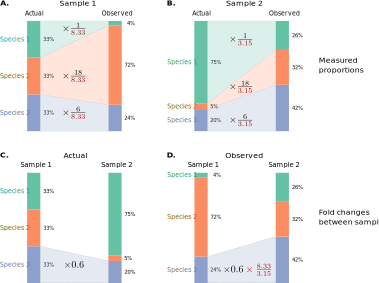
\includegraphics[width=0.9\linewidth]{figures/export-pdf/figures/illustrations/error-proportions} \caption{\textbf{Taxonomic bias creates sample-dependent multiplicative errors in species proportions, which can lead to inaccurate fold changes between samples.} Top row: Error in proportions measured by MGS in two hypothetical microbiome samples that contain different relative abundances of three species. Bottom row: Error in the measured fold-change in the third species that is derived from these measurements. Species' proportions may be measured as too high or too low depending on sample composition. For instance, Species 3 has an efficiency of 6 and is under-measured in Sample 1 (which has a mean efficiency of 8.33) but over-measured in Sample 2 (which has a mean efficiency of 3.15).}\label{fig:error-proportions}
\end{figure}



\textbf{Higher-order taxa:} How does bias affect the proportions and ratios of higher-order taxa, such as a genera, phyla, or even all organisms?
More generally, we can identify an higher-order taxon \(I\) with a set of species, \(\{i \in I\}\).
The abundance and reads of a taxon \(I\) in a sample \(a\) equal the sums over its constituent species, \(\text{abun}_{I}(a) = \sum_{i \in I}\text{abun}_{i}(a)\) and \(\text{reads}_{I}(a) = \sum_{i \in I}\text{reads}_{i}(a)\).
The efficiency of taxon \(I\) equals the weighted average of its constituent species,
\begin{align}
  \label{eq:efficiency-general}
  \text{efficiency}_I(a) 
    \equiv \frac{\sum_{i\in I}\text{abun}_i(a)\cdot \text{efficiency}_i}{\text{abun}_I(a)}.
\end{align}
Thus the efficiency of a higher-level taxon may vary across samples (McLaren, Willis, and Callahan (\protect\hyperlink{ref-mclaren2019cons}{2019})).
An exception is if the constituent species have the same efficiency or always appear in the same abundances relative to each other, in which case the efficiency of the higher-order taxon would stay constant.
As an example, suppose that Species 1 and Species 2 in Figure \ref{fig:error-proportions} were in the same phylum.
The efficiency of the phylum would then be \(\tfrac{1}{2} \cdot 1 + \tfrac{1}{2} \cdot 18 = 9.5\) in Sample 1 and \(\tfrac{15}{16} \cdot 1 + \tfrac{1}{16} \cdot 18 \approx 2.1\) in Sample 2.
Equations \eqref{eq:prop-error} and \eqref{eq:ratio-error} continue to describe the measurement error in proportions and ratios involving higher-order taxa, so long as the sample-dependent taxon efficiency defined by Equation \eqref{eq:efficiency-general} is used.
In this way, we can see that both proportions and ratios among higher-order taxa may have inconsistent fold errors.

\hypertarget{absolute-abundance}{%
\subsection{Absolute abundance}\label{absolute-abundance}}

Various methods can be used to convert the relative abundances from MGS into absolute abundances.
These methods are subject to taxonomic bias in the MGS measurements and in any supplemental, non-MGS measurements that may be used for the conversion.
Appendix {[}REF{]} develops a general framework to understand how bias affects absolute-abundance measurements for species and higher-order taxa across these methods.
Here we present our main results as they apply to currently-used methods.

\hypertarget{methods-that-measure-total-community-abundance}{%
\subsubsection{Methods that measure total-community abundance}\label{methods-that-measure-total-community-abundance}}

The definition \eqref{eq:prop} for the proportion of a species indicates that we can convert proportions to absolute abundances were we to know the absolute abundance of the total community.
Given our measured proportions from MGS and a measure of total abundance from a supplemental, non-MGS measurement, \(\widehat{\text{abun}}_{S}(a)\), one can measure the abundances of individual species by
\begin{align}
  \label{eq:density-prop-meas}
  \widehat{\text{abun}}_{i}(a) 
  &= \widehat{\text{prop}}_{i}(a) \cdot \widehat{\text{abun}}_S(a).
\end{align}
Total-abundance measurements that have recently used for this purpose include counting cells with microscopy (Lloyd et al. (\protect\hyperlink{ref-lloyd2020evid}{2020})) or flow cytometry (Props et al. (\protect\hyperlink{ref-props2017abso}{2017}),Vandeputte et al. (\protect\hyperlink{ref-vandeputte2017quan}{2017}),Galazzo et al. (\protect\hyperlink{ref-galazzo2020howt}{2020})), measuring the concentration of a marker-gene with qPCR or ddPCR (Zhang et al. (\protect\hyperlink{ref-zhang2017soil}{2017}),Barlow, Bogatyrev, and Ismagilov (\protect\hyperlink{ref-barlow2020aqau}{2020}), Galazzo et al. (\protect\hyperlink{ref-galazzo2020howt}{2020}),Tettamanti Boshier et al. (\protect\hyperlink{ref-tettamantiboshier2020comp}{2020})), and measuring bulk DNA concentration with a florescence-based DNA quantification method (Contijoch et al. (\protect\hyperlink{ref-contijoch2019gutm}{2019})).

Importantly, these methods of measuring total abundance are themselves subject to taxonomic bias.
Flow cytometry may, for example, yield lower cell counts for species whose cells tend to clump together or are prone to lysis during steps involved in sample collection, storage, and preparation.
The marker-gene concentration measured by qPCR is affected by variation among species in extraction efficiency, marker-gene copy number, and PCR binding and amplification efficiency.
We can easily understand the impact of taxonomic bias on the total-abundance measurement under simplifying assumptions analogous to those in our MGS model.
Suppose that each species has an \emph{absolute efficiency} for the total-abundance measurement that is constant across samples.
Neglecting other sources of random and systematic error, the total-abundance measurement equals
\begin{align}
  \label{eq:total-density-error}
  \widehat{\text{abun}}_S(a) 
  &= \sum_{i\in S} \text{abun}_i(a) \cdot \text{efficiency}^{\text{tot}}_i
\\&= \text{abun}_S(a) \cdot \text{efficiency}^{\text{tot}}_S(a),
\end{align}
where \(\text{efficiency}_{i}^{\text{tot}}(a)\) is the absolute measurement efficiency of species \(i\) for the total-abundance measurement and \(\text{efficiency}^{\text{tot}}_S(a)\) is the mean efficiency of the total-abundance measurement in the sample.

The species abundance measurements are affected by taxonomic bias in both the MGS and total-abundance measurement.
We can compute this effect by substituting Equations \eqref{eq:prop-error} and \eqref{eq:total-density-error} into Equation \eqref{eq:density-prop-meas}, yielding
\begin{align}
  \label{eq:density-prop-error}
  \widehat{\text{abun}}_{i}(a) 
  = \text{abun}_{i}(a) \cdot \frac{\text{efficiency}_{i} \cdot \text{efficiency}^{\text{tot}}_S(a)}{\text{efficiency}_S(a)}.
\end{align}
Equation \eqref{eq:density-prop-error} indicates that the multiplicative error in the measured absolute abundance of a species equals its MGS efficiency relative to the mean MGS efficiency in the sample, multiplied by the mean efficiency of the total measurement.
As in the case of proportions (Equation \eqref{eq:prop-error}), the error depends on sample composition through the two mean efficiency terms and so may vary across samples.
On the other hand, if the mean efficiency of the total-abundance measurement mirrors that of the MGS measurement, the two can offset and lead to more stable errors.
We discuss how this possibility might be exploited in real experimental workflows in Section \ref{solutions}.

\hypertarget{methods-that-determine-or-measure-a-reference-species}{%
\subsubsection{Methods that determine or measure a reference species}\label{methods-that-determine-or-measure-a-reference-species}}

The definition \eqref{eq:ratio} for the ratio between two species suggests another method to convert relative to absolute abundances:
By knowing the ratio of species \(i\) to a \emph{reference species} \(r\) and the abundance of species \(r\), we can determine the abundance of species \(i\).
Thus given an MGS measurement and a measurement \(\widehat{\text{abun}}_{r}(a)\) of the abundance of species \(r\), we can measure the abundance of an arbitrary species \(i\) as
\begin{align}
  \label{eq:density-ratio-meas}
  \widehat{\text{abun}}_{i}(a) = \text{reads}_{i}(a) \cdot \frac{\widehat{\text{abun}}_{r}(a)}{\text{reads}_{r}(a)}.
\end{align}
Here we consider some practical applications of this method and how their measurements are affected by bias in the MGS measurement and error in \(\widehat{\text{abun}}_{r}(a)\).
Appendix {[}REF{]} describes the general case where there is a set \(R\) of multiple reference species; here we restrict our attention to a single reference species \(r\).

This approach has so far been solely or primarily used with reference species that have been determined to have an abundance that is constant across samples.
In a spike-in experiment, researchers deliberately add (or `spike in') one or more reference species at a known, constant abundance.
For a single spike-in species \(r\), the abundances of other species can be estimated by Equation \eqref{eq:density-ratio-meas}.
In the absence of spike-ins, researchers may be able to determine one or more native species whose abundances are thought to be constant across samples; we refer to such species as \emph{housekeeping species} by analogy with the housekeeping genes used for absolute-abundance conversion in studies of gene expression.
Housekeeping species can sometimes be identified using prior scientific knowledge; for example, in shotgun sequencing experiments, researchers have used sequencing reads from the plant or animal host as a reference.
A related approach involves computationally identifying species that are constant between pairs of samples (David et al. (\protect\hyperlink{ref-david2014host}{2014})) or between sample conditions (Mandal et al. (\protect\hyperlink{ref-mandal2015anal}{2015}), Kumar et al. (\protect\hyperlink{ref-kumar2018anal}{2018})) under added statistical assumptions about the existence of such species.
The abundance of a housekeeping species is typically unknown; therefore, to estimate the abundances of other species, we simply set \(\widehat{\text{abun}}_{r}(a)\) to 1 in Equation \eqref{eq:density-ratio-meas}.
The resulting abundance measurements have unknown but fixed units, which is sufficient for measuring fold changes across samples.

Equation \eqref{eq:density-ratio-meas} makes clear that the reference species need not be constant so long as we can directly measure it.
This observation suggests a new approach to obtaining species absolute abundances, by combining MGS measurements of the community with targeted measurements of the absolute abundance of one or more individual species.
Common targeted measurements include using qPCR or ddPCR to measure the concentration of a marker-gene in the extracted DNA, using primers tailored to a particular species.
Other methods that are capable of measuring cells (rather than extracted DNA) include applying ddPCR directly to cells, performing CFU counting on selective media, and using flow cytometry with species-specific florescent probes.
The measurements from any of these methods could be used for \(\widehat{\text{abun}}_{r}(a)\) in Equation \eqref{eq:density-ratio-meas} to obtain the absolute abundance for all species.
Appendix {[}REF{]} describes how using multiple reference species and/or statistical modeling can address the fact that any one native reference species is unlikely to be found in all samples.

Despite the diversity of these methods, each can be represented by Equation \label{eq:density-ratio-meas}, making it straightforward to understand the impact of taxonomic bias in the MGS measurement.
It follows from Equation \eqref{eq:ratio-error} that the measured abundance of species \(i\) is
\begin{align}
  \label{eq:density-ratio-error}
  \widehat{\text{abun}}_{i}(a) 
  = \text{abun}_{i}(a) \cdot \frac{\text{efficiency}_{i}}{\text{efficiency}_{r}}
  \cdot \underbrace{\frac{\widehat{\text{abun}_r}(a)}{\text{abun}_r(a)}}_{\substack{\text{fold error in} \\ \text{ref. species}}}.
  % \cdot \begin{array}{c} \text{fold error in} \\ \widehat{\text{abun}_r}(a) 
\end{align}
The error thus consists of two terms: the ratio of the efficiency between species \(i\) and species \(r\), and any error in the abundance of the reference species.
The ratio of species efficiencies is constant by assumption; thus the total error is constant if the error in the reference abundance is.
Note, if a higher-order taxon is used as a reference---for example, using targeted measurements of a genus or family---then the efficiency of the reference taxon may vary across samples, leading to non-proportional errors.

In practice, researchers commonly use a less-direct but equivalent approach to measure species abundances from a reference such as a spike-in.
Set \(S\) to be the species of interest excluding the spike-in species \(r\).
In this approach, one measures the total abundance of the community \(S\) from the ratio of non-spike-in to spike-in reads,
\begin{align}
  \label{eq:total-density-spike}
  \widehat{\text{abun}}_S(a) 
  &= \frac{\text{reads}_S(a) \cdot \widehat{\text{abun}}_R(a)}{\text{reads}_r(a)}.
\end{align}
Then, one uses this measurement \(\widehat{\text{abun}}_{S}(a)\) along with the MGS proportions in Equation \eqref{eq:density-prop-meas} to determine the abundance of individual species.
This calculation yields measurements that are identical to those from directly applying Equation \eqref{eq:density-ratio-meas} (Appendix \ref{total-density-ref}).
This observation might seem paradoxical: Equation \eqref{eq:density-ratio-error} indicates proportional error for the direct approach, whereas \eqref{eq:density-prop-error} suggests non-proportional errors for the indirect approach.
This apparent contradiction is resolved by the fact the measurement \(\widehat{\text{abun}}_{S}(a)\) by this method has errors that are proportional to \(\text{efficiency}_S(a)\) and thus exactly offset the proportionality with \(1/\text{efficiency}_S(a)\) in the MGS proportions, such that the measured species abundances have constant fold errors.

\hypertarget{summary}{%
\subsection{Summary}\label{summary}}

Taxonomic bias in MGS measurements makes all MGS-based measures of relative and absolute abundance inaccurate.
For some measures---but not all---consistent bias at the species level creates proportional errors in species abundances.
Of two types of relative abundance, the ratio between a pair of species has proportional errors whereas the proportion of an individual species does not.
Instead, the multiplicative error in a species' proportion varies with the mean efficiency across samples.
Methods for measuring species absolute abundance that involve measuring the abundance of the total community likewise experience non-proportional errors which vary with the sample mean efficiency;
a notable exception is if the mean efficiency of the total-abundance measurement mirrors that of the MGS measurement.
Absolute-abundance methods that instead involve measuring or spiking individual reference species yield proportional errors, provided that the abundance of the reference species can be determined up to a proportional error.
The efficiency of higher-order taxa may vary across samples even if the efficiencies of their constituent species are constant; as a result, all standard abundance measures can have non-proportional errors at taxonomic resolutions higher than that at which bias is conserved.

\hypertarget{differential-abundance}{%
\section{DA methods vary in their robustness to bias}\label{differential-abundance}}

This section turns to how these errors in individual sample measurements described in the previous section affect the results of cross-sample comparisons and DA analyses of many samples.
Microbiome researchers employ many measures for the change in species' abundance across samples.
We focus on analyses of multiplicative or (log) fold changes, which are common across study types and have more direct ecological interpretations than other measures (via the processes of exponential growth and decay).
In addition, we briefly consider non-parametric rank-based analyses that are common in microbiome-wide association studies.

\hypertarget{fold-changes-between-a-pair-of-samples}{%
\subsection{Fold changes between a pair of samples}\label{fold-changes-between-a-pair-of-samples}}

The building blocks of a multiplicative DA analysis are the fold changes (FCs) in abundance between individual pairs of samples.
Intuitively, only abundance measurements that have proportional errors will have FCs that are completely robust to bias.

The phenomenon by which non-proportional errors due to bias distort measured FCs can be seen most simply for species proportions.
It follows from Equation \eqref{eq:prop-error} that the measured FC in the proportion of a species \(i\) from samples \(a\) to \(b\) is
\begin{align}
  \label{eq:prop-fc-error}
\underbrace{\frac{\widehat{\text{prop}}_{i}(b)}{\widehat{\text{prop}}_{i}(a)}} _\text{measured FC}
  &= \frac
    {\text{prop}_{i}(b) \cdot \cancel{\text{efficiency}_{i}} / {\text{efficiency}_S(b)}}
    {\text{prop}_{i}(a) \cdot \cancel{\text{efficiency}_{i}} / {\text{efficiency}_S(a)}}
\\[0.5ex]
  &=
  \underbrace{\frac{\text{prop}_{i}(b)}{\text{prop}_{i}(a)}}_\text{actual FC}
  \cdot
  \underbrace{\left[\frac{\text{efficiency}_S(b)}{\text{efficiency}_S(a)}\right]^{-1}}_\text{fold error}
  .
\end{align}
The sample-independent efficiency factor cancels, but the sample-dependent mean efficiency does not, leaving an error in the measured FC equal to the inverse change in mean efficiency.
In contrast, the ratio between species \(i\) and \(j\) has proportional error and so its FC is unaffected by bias.
From Equation \eqref{eq:ratio-error},
\begin{align}
  \label{eq:ratio-fc-error}
\underbrace{\frac{\widehat{\text{ratio}}_{i/j}(b)}{\widehat{\text{ratio}}_{i/j}(a)}} _\text{measured FC}
  &= \frac
    {\text{ratio}_{i/j}(b) \cdot \cancel{\text{efficiency}_{i} / {\text{efficiency}_j}}}
    {\text{ratio}_{i/j}(a) \cdot \cancel{\text{efficiency}_{i} / {\text{efficiency}_j}}}
\\[0.5ex]
  &=
  \underbrace{\frac{\text{ratio}_{i/j}(b)}{\text{ratio}_{i/j}(a)}}_\text{actual FC}
  ;
\end{align}
the constant error, equal to the ratio between the species' efficiencies, completely cancels, leaving an accurately measured FC.

Figure \ref{fig:error-proportions} (bottom row) illustrates these two different behaviors for the error in the FCs of proportions versus ratios when the mean efficiency varies between samples.
Here the mean efficiency decreases by a factor of 2.6 (FC of 0.4X) from Sample 1 to Sample 2, which causes the FC of the proportion of each species to be measured as 2.6X larger than its true value.
Though the fold error for all species is the same, the implications depend on the actual FC and correspond to three distinct types of error: an increase in magnitude, a decrease in magnitude, and a change in direction; we refer to the latter as a \emph{sign error} in reference to the corresponding log fold change (LFC).
We can see each type of error in Figure \ref{fig:error-proportions}.
For Species 1, which increases and thus moves in the opposite direction of the mean efficiency, we see an increase in magnitude of the measured FC (actual FC: 2.3X, measured FC: 6.5X).
For Species 2, which decreases and thus moves in the same direction as the mean efficiency but by a larger factor, we see an decrease in magnitude (actual FC: 0.15X, measured FC: 0.44X).
For Species 2, which decreases by a smaller factor than the mean efficiency, we see a change in direction (actual FC: 0.6X, measured FC: 1.8X), such that the species actually appears to increase (a sign error).
In contrast, the fold error in Equation \eqref{eq:ratio-error} completely cancels when we divide the ratio measured for one sample \(a\) by another sample \(b\).

Absolute-abundance measurements for which bias creates non-proportional errors are subject to the same limitation as proportions.
In particular, abundance measured by normalization of MGS proportions to a total-abundance measurement will yield errors in FCs given by the inverse change in the mean efficiency, unless this change is offset by error in the total-abundance measurement itself.
On the other hand, abundances measured by normalization to one or more reference species are capable of having proportional errors that cancel in FC calculations.

\hypertarget{regression-analysis-of-many-samples}{%
\subsection{Regression analysis of many samples}\label{regression-analysis-of-many-samples}}

DA analysis of multiple samples can be framed as a regression problem in which we analyze the relationship between a microbial \emph{response variable}, such as the log abundance of species \(i\), with one or more \emph{covariates}, such as the pH of the sampled environment or whether the sample is from a healthy or sick person.
The simplest regression analysis uses the simple linear regression model,
\begin{align}
  \label{eq:regression}
  \log \widehat{\text{abun}}_i(a) = \alpha_i + \beta_i x(a) + \varepsilon_i(a),
\end{align}
where \(x\) is a continuous covariate (e.g.~pH) or a binary covariate (e.g.~\(x=1\) for treated patients and \(x=0\) for controls), \(\alpha_i\) and \(\beta_i\) are regression coefficients, and \(\varepsilon_i(a)\) is a mean-zero random variable that reflects the residual (unexplained) variation in the response.
In a DA analysis, we are interested in the slope coefficient \(\beta\), which describes how the species' abundance changes with \(x\).
We are generally uninterested in the intercept coefficient, \(\alpha\), which captures differences in the baseline abundance among species and---it is usually hoped---study- and species-specific systematic error such as that created by taxonomic bias.

How does taxonomic bias in fact impact estimates of the slope coefficient, \(\beta\)?
Appendix \ref{appendix-regression} derives the effect of bias on the estimated coefficients for the simple linear regression model under estimation via Ordinary Least Squares (OLS) or Maximum Likelihood Estimation (MLE).
The result has a simple interpretation that provides intuition for what to expect in more complicated generalized linear regression models used in popular DA methods.
Consider the regression \eqref{eq:regression} fit to the measured log abundance of species \(i\) across all samples.
The measurement error in the response variable,
\begin{align}
  \text{error}_{i}(a) \equiv 
  \log \widehat{\text{abun}}_i(a) - \log \text{abun}_i(a)
  = \log \frac{\widehat{\text{abun}}_i(a)}{\text{abun}_i(a)},
\end{align}
can be thought of as having three components:

\begin{itemize}
\tightlist
\item
  Error that is constant across samples affects the intercept coefficient, \(\alpha_i\).
\item
  Error that varies systematically with \(x\) affects the slope coefficient, \(\beta_i\).
\item
  Error that varies and is uncorrelated with \(x\) affects the residual variation, \(\varepsilon_{i}(s)\).
\end{itemize}

We saw in Section \ref{abundance-measurement} that the error from taxonomic bias has a species-specific, sample-independent component that is constant across samples; this component causes a species-specific systematic error in the estimated intercept, \(\alpha_{i}\).
The error also has a sample-specific, species-independent component.
The portion that is correlated with the covariate \(x\) creates a systematic error in the slope coefficient \(\beta_{i}\) that is the same for every species and opposite in sign to how the error varies with \(x\);
the portion that is uncorrelated with \(x\) affects the precision (standard errors) of the slope estimates in a species-specific manor.

Figure \ref{fig:regression-example} illustrates with a simulated data for the case of log abundance measured using the total-abundance normalization method (Equation \eqref{eq:density-prop-meas}), assuming that total community abundance is measured perfectly accurately.
In this case, the variable component of the error is due entirely to variation in the log mean efficiency of the MGS measurement.
Variation in the log mean efficiency that is associated with the covariate \(x\) creates a systematic error in the estimated slope \(\hat \beta\) equal to the negative of the (scaled) covariance of log mean efficiency with \(x\).
The absolute error is the same for all species; however, its relative value depends on the magnitude of the covariance of the log mean efficiency with \(x\) relative to that of the response (here, \(\log \text{abun}_{i}\)) with \(x\) or, equivalently, the relative magnitudes of their slopes.
As in the case of fold changes between pairs of samples, the net effect can be decreases in magnitude (Species 9, 10, and 1 in Figure \ref{fig:regression-example}), changes in sign (Species 5), or increases in magnitude (remaining species) depending on these relative values.
Variation in the log mean efficiency that is uncorrelated with \(x\) does not systematically distort \(\hat \beta\) but does affect its precision, typically leading to increased standard errors as the variation in log mean efficiency effectively acts as an additional source of noise in measured abundance (Figure \ref{fig:regression-example} D).
The exception is for species whose residual variation is strongly positively correlated with that of log mean efficiency (here, Species 9), which can appear to have less random variation and receive standard errors that are too small.
Decreased magnitudes and increased standard errors can both cause associations to be missed that would otherwise have been detected (Species 10 and 1), while increased magnitudes can turn weak or statistically insignificant associations into strong and statistically significant ones (Species 7, 6 and 4).

Overall, we find that variation in measurement error created by variation in the mean efficiency of the MGS measurement can negatively affect certain DA analyses by creating systematic errors in the slope coefficient estimates and/or reducing their precision.
Similar effects occur for regressions of log proportions and of log abundances derived by total-abundance normalization when the total abundance is accurately measured; however, as noted in Section \ref{abundance-measurement}, total-abundance measurements that are taxonomically biased in a complementary manner can mitigate these effects.
Regression analyses of log-ratios and log abundances derived from reference-species normalization remain unaffected---the errors are constant across samples and so only impact the intercept coefficients.

\begin{figure}
\centering
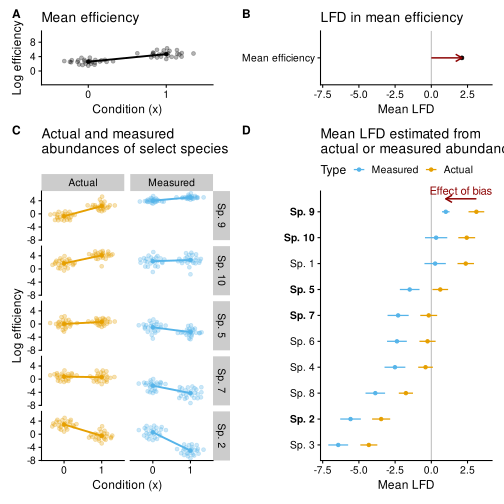
\includegraphics{figures/export-pdf/home/michael/research/differential-abundance-theory/notebook/_posts/2021-08-03-simulate-regression-example/simulate-regression-example_files/figure-html5/main-figure-1.pdf}
\caption{\label{fig:regression-example}\textbf{Taxonomic bias distorts multi-sample differential abundance inference when the mean efficiency of samples is associated with the covariate of interest.} This figure shows the results of a regression analysis of simulated microbiomes consisting of 50 samples and 10 species from two environmental conditions indexed by \(x=0\) and \(x=1\). In this simulation, the species with the largest efficiency (Species 9) also has the largest positive LFC, which drives the positive association of the log mean efficiency with the condition (shown in Panels A and B). This positive LFC in the log mean efficiency induces a systematic negative shift in the estimated LFCs of all species (Panels C and D). Panel D shows the mean LFC (points) with 95\% confidence intervals (CIs), for each species estimated from either the actual or the measured densities. The error (difference in LFC estimates on measured and actual) equals the negative LFC of the mean efficiency (shown in Panel B).}
\end{figure}



\hypertarget{todo-rank-based-analyses}{%
\subsubsection{{[}TODO{]} Rank-based analyses}\label{todo-rank-based-analyses}}

\hypertarget{case-studies}{%
\section{Case studies ~}\label{case-studies}}

To better understand the potential impact of taxonomic bias on DA analysis in practice, we conducted several case studies spanning a range of biological scenarios and sequencing technologies.

\hypertarget{foliar-fungi-experiment}{%
\subsection{Foliar fungi experiment}\label{foliar-fungi-experiment}}

The taxonomic bias species present in `mock communities' of known composition can be directly measured, and the measured bias can then be used to correct downstream DA analysis (McLaren, Willis, and Callahan (\protect\hyperlink{ref-mclaren2019cons}{2019})).
In practice it is difficult to construct control communities that span the many species present in complex natural communities.
However, gnotobiotic community experiments are well suited to this form of \emph{calibration via community controls} since, unlike most natural ecosystems, it is possible to assemble mock communities containing all species in known relative abundances.

In a study of host-commensal-pathogen interactions, Leopold and Busby (\protect\hyperlink{ref-leopold2020host}{2020}) inoculated plants with 8 commensal fungal species and subsequently exposed plants to a fungal pathogen.
The authors used ITS amplicon sequencing to measure communities before and after pathogen infection.
Motivated by the substantial ribosomal copy-number variation (CNV) in fungi (Lofgren et al. (\protect\hyperlink{ref-lofgren2019geno}{2019})), the authors also performed control measurements of mock communities that they constructed from quantified genomic DNA of the 9 species in the experiment; these controls were used to measure taxonomic bias with the method of McLaren, Willis, and Callahan (\protect\hyperlink{ref-mclaren2019cons}{2019}).
The authors found a 13X difference between the most and least efficiently measured commensal, while the pathogen was measured 40X more efficiently than the least efficiently measured commensal.

Leopold and Busby (\protect\hyperlink{ref-leopold2020host}{2020}) performed two related DA analyses on the pre-infection communities: the first characterized the relative importance of host genetics and species arrival order on species relative abundances in the fully-established community, and the second quantified the strength of `priority effects'---the advantage gained by a species from being allowed to colonize first.
Both analyses were based on fold changes in species proportions and so in principle were sensitive to taxonomic bias.
To improve accuracy, the authors incorporated the bias measured from the control samples with analysis-specific calibration procedures.

We repeated the two DA analyses of Leopold and Busby (\protect\hyperlink{ref-leopold2020host}{2020}) with and without calibration and found that the results did not meaningfully differ.
To understand why, we examined the variation in species proportions and the mean efficiency across the pre-infection communities (SI Figure \ref{fig:leopold2020host-variation}).
Despite the 13X variation in the efficiencies among species, the mean efficiency hardly varied across samples (SI Figure \ref{fig:leopold2020host-variation}C), having a geometric range of 1.62X and a geometric standard deviation of 1.05X.
This consistency in the mean efficiency was despite the fact that each species each showed substantial multiplicative variation (SI Figure \ref{fig:leopold2020host-variation}A).
But the pre-infection samples were always dominated by the three species with the highest efficiencies, which varied by 3X and by just 1.5X between the two most dominant.
The mean efficiency, equal to the proportion-weighted arithmetic average of species efficiencies, is insensitive to species present at low relative abundance and so remained relatively constant across samples.
Because the multiplicative variation in the mean efficiency was much smaller than that in the proportions of individual taxa, it had a negligible impact on the inferred fold changes and the DA analyses based on them.

We performed an additional DA analysis on the data from Leopold and Busby (\protect\hyperlink{ref-leopold2020host}{2020}) to investigate whether any commensals increased in absolute concentration in response to infection.
The pathogen is absent in pre-infection samples but tends to dominate the community post-infection, resulting in a substantially higher mean efficiency in post-infection samples (SI Figure \ref{fig:leopold2020host-infection-mean-efficiency-dist}).
Across different host genotypes, the average post-infection increase in mean efficiency ranged from 2.5X to 5.2X.
We used simple linear regression to measure the LFC in commensal species proportions pre- to post-infection, with and without calibration (SI Figure \ref{fig:leopold2020host-infection-lfc}).
All commensals tended to decrease in proportion post-infection, which is expected given the pathogen's growth to most abundant community member and the sum-to-one constraint of species proportions.
However, when taxonomic bias was ignored the magnitude of the post-infection decrease was overestimated, by an amount corresponding to the inverse change in log mean efficiency.
This magnitude error was substantial for the commensal-host pairs with the weakest changes; in several cases, LFC estimates with 95\% confidence intervals below 0 became indistinguishable from 0 after calibration.

Although Leopold and Busby (\protect\hyperlink{ref-leopold2020host}{2020}) did not include absolute-abundance measurements, we can consider the impact taxonomic bias would have on an absolute DA analysis in a simple scenario in which total genome concentration of each pre- and post-infection sample is perfectly known.
The total genomic concentrations of each sample, combined with the species proportions measured by MGS, can be combined into a measurement of species concentrations using the total-abundance normalization method (Equation \eqref{eq:density-prop-meas}).
In this case, the bias in the MGS measurements will create absolute errors in the estimated LFCs of genome concentration of equal magnitude to the errors in the LFC estimates for proportions.
The scientific error, however, might become worse.
Suppose that the species whose calibrated proportions appeared to hold steady or slightly decrease actually increased in absolute abundance by around 2X.
As bias shifts our estimates downwards by 2.5X to 5.2X, we would instead conclude that these taxa decreased.

\hypertarget{vaginal-microbiomes-of-pregnant-women}{%
\subsection{Vaginal microbiomes of pregnant women}\label{vaginal-microbiomes-of-pregnant-women}}

The vaginal microbiome during pregnancy has been a source of intensive study due to its apparent connection with the health of both mother and her developing child.
Many MGS studies have found associations of specific microbial species and community characteristics with rates of urinary tract and sexually-transmitted infections, bacterial vaginosis (BV), and preterm birth.
Yet these associations vary across studies of different populations and using different MGS methods.
DA analyses of the vaginal microbiome are commonly based on proportions, creating an opportunity for taxonomic bias to impact results.
A number of studies have experimentally demonstrated substantial taxonomic bias among MGS protocols and individual steps (such as extraction and PCR amplification) in vaginal samples or \emph{in vitro} samples of vaginally-associated species (Yuan et al. (\protect\hyperlink{ref-yuan2012eval}{2012}),Brooks et al. (\protect\hyperlink{ref-brooks2015thet}{2015}),Gill et al. (\protect\hyperlink{ref-gill2016eval}{2016}),Graspeuntner et al. (\protect\hyperlink{ref-graspeuntner2018sele}{2018})).
Bias has been proposed as a potential explanation for discrepancies across studies (Callahan et al. (\protect\hyperlink{ref-callahan2017repl}{2017}), Others?), but there has so far been little quantitative analysis of this possibility.
Here we use empirical bias measurements from control samples to investigate the role of bias in proportion-based DA analyses of vaginal microbiomes from a recent large-cohort study of pregnant women.

As part of the Multi-Omic Microbiome Study: Pregnancy Initiative (MOMS-PI) study, Fettweis et al. (\protect\hyperlink{ref-fettweis2019thev}{2019}) collected longitudinal samples from over 1500 pregnant women, including nearly 600 that were measured by amplicon sequencing of the 16S V1-V3 hypervariable region to yield species-level bacterial taxonomic profiles.
Taxonomic bias of this MGS protocol was previously investigated by Brooks et al. (\protect\hyperlink{ref-brooks2015thet}{2015}) and McLaren, Willis, and Callahan (\protect\hyperlink{ref-mclaren2019cons}{2019}), using measurements by Brooks et al. (\protect\hyperlink{ref-brooks2015thet}{2015}) of cellular mock communities of seven common, clinically-relevant vaginal bacterial species.
Of these, \emph{Lactobacillus iners} had the highest efficiency, which was nearly 30X larger than that of the species with the lowest efficiency, \emph{Gardnerella vaginalis}.
A second \emph{Lactobacillus} species, \emph{L. crispatus}, had an efficiency that was approximately 2X less than \emph{L. iners} and 15X greater than \emph{G. vaginalis}.
These species, along with the unculturable \emph{Lachnospiraceae BVAB1}, are the most common top (most-abundant) species (SI analysis) and can reach high proportions in individual samples, indicating that shifts between them might drive large changes in the mean efficiency which might in turn impact DA results.

We sought to assess this possibility using a joint analysis of the control measurements from Brooks et al. (\protect\hyperlink{ref-brooks2015thet}{2015}) and the microbiome measurements from the MOMS-PI study.
To obtain the taxonomic bias among all species identified in the MOMS-PI measurements, we used the taxonomic relationships with the seven control species to impute the efficiencies for the remaining species.
We used these imputed efficiencies to calibrate (correct the effect of bias in) the MOMS-PI measurements, examine variation in the mean efficiency varied across samples, and compare the results of a DA analysis with and without bias correction.

The mean efficiency varies substantially across vaginal samples (Figure \ref{fig:momspi-mean-efficiency-dist}.
This variation appears to be primarily driven by variation in which species is most abundant, samples in which a \emph{Lactobacillus} species is most abundant (after calibration) typically have an efficiency that is 3-20X greater than samples in which \emph{G. vaginalis} is most abundant.
Shifts between \emph{Lactobacillus}-dominance and \emph{Gardnerella}-dominance are common in between-women comparisons and occasionally occur between consecutive visits in individual women (SI Figure \ref{fig:momspi-mean-efficiency-fcs}).
These shifts typically result in substantial fold changes in mean efficiency (SI Figure \ref{fig:momspi-mean-efficiency-fcs}) and can cause spurious fold changes in the trajectories of lower-abundance species (SI Figure \ref{fig:momspi-trajectory}).
Decreases in mean efficiency during transitions from \emph{Lactobacillus} to \emph{Gardnerella} dominance would be more extreme for vaginal microbiome primer sets that fail to amplify \emph{Gardnerella} (Graspeuntner et al. (\protect\hyperlink{ref-graspeuntner2018sele}{2018})).

\begin{figure}
\centering
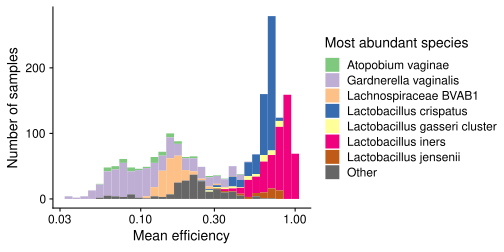
\includegraphics{figures/export-pdf/notebook/_posts/2021-11-01-momspi-summary/momspi-summary_files/figure-html5/momspi-mean-efficiency-dist-1.pdf}
\caption{\label{fig:momspi-mean-efficiency-dist}\textbf{The mean efficiency in vaginal samples from the MOMS-PI study varies with the most abundant species.}}
\end{figure}



We next considered whether the observed variation in mean efficiency could cause systematic error in a DA analysis.
In particular, we hypothesized that DA analysis of species proportions versus a covariate that is associated with \emph{Lactobacillus} and/or \emph{Gardnerella} would be particularly prone to spurious results.
Patient metadata was not available due to privacy restrictions; we therefore sought a clinically relevant covariate to use in a regression analysis that could be determined directly from the microbiome profiles and that we \emph{a priori} expected to be associated with the proportions of \emph{Lactobacillus} and \emph{Gardnerella}.
Alpha diversity metrics such as species richness, the Shannon index, and the (Inverse) Simpson index have been repeatedly found to be strongly positively associated with bacterial vaginosis (BV; Srinivasan et al. (\protect\hyperlink{ref-srinivasan2012bact}{2012}), Cartwright et al. (\protect\hyperlink{ref-cartwright2018mult}{2018})).\footnote{Cartwright et al. (\protect\hyperlink{ref-cartwright2018mult}{2018}) found that an observed Simpson Diversity Index of 0.82 (corresponding to an order-2 effective number of species of 5.6) classified high diversity samples as BV positive with a sensitivity of 100\% and specificity of 85.1\%.}
In addition, it is commonly observed that samples from women with and without BV that are dominated by \emph{Lactobacillus spp.} tend to have higher diversity, whereas samples dominated by \emph{Gardnerella} tend to have lower diversity.
We therefore chose to perform a DA analysis of species proportion versus alpha diversity, hypothesizing that \emph{Lactobacillus} and \emph{Gardnerella} would drive a negative association of mean efficiency with diversity and thereby distort DA estimates for all species.
We split samples into low, medium, and high diversity groups based on Shannon diversity in observed (uncalibrated) microbiome profiles.
We then estimated the LFC in proportion from low- to high-diversity samples for 30 species passing a basic prevalence threshold, with and without bias correction.
A large fraction of entries in the species count matrix were small counts or zeros.
We used therefore used gamma-Poisson (or negative-binomial) regression of the observed read counts to fit a linear model to log species proportions while accounting for uncertainty from the random sampling of reads.
We accounted for bias by including an offset term in the linear model equal to the log ratio of the species' efficiency to the sample mean efficiency.

The mean efficiency was on average lower in high-diversity samples due to a reduction in \emph{Lactobacillus} dominance (LFC of -1.6, or a 4.8X reduction).
Our results from the previous section therefore suggest that accounting for bias should reduce the estimated LFC for each species by about this same amount.
We found that, as expected, bias correction reduced the LFC of each species, though the effect was variable and typically somewhat smaller.
Bias correction led to substantial magnitude changes for several species and sign changes in 3 species; however, the relative difference between the corrected and uncorrected LFCs was modest for the 19/30 species with the largest LFCs of over 2 (corresponding to a FC of 7.4X) even after correction.
These large LFCs occur in species that rarely if ever reach high proportions and so are likely driven by the sum-to-one constraint: The high diversity communities are those not dominated by \emph{Lactobacillus} spp. (or to a lesser extent \emph{G. vaginalis} and BVAB1).
Therefore it is not clear how well it will generalize to regressions on other covariates.

\hypertarget{human-gut-microbiomes}{%
\subsection{Human gut microbiomes}\label{human-gut-microbiomes}}

An overwhelming majority of applications of DA analysis are in studies of the human gut microbiome. (True?)
Many are microbial association tests in a case-control design---looking for taxa that are differentially abundant in one group of subjects versus another.
It is also increasingly common to perform time series experiments to elucidate dynamics of microbial communities within a host and their interaction with dynamic host variables.
Although interest in other microorganisms and viruses is growing, so far these are mostly of bacteria.
Were therefore asked whether there are features of human gut bacterial microbiomes that we might expect to make DA analyses more or less robust to taxonomic bias.

We first considered whether the greater diversity of the human gut microbiome as compared to the human vaginal microbiome might limit the impact of bias on species-level DA analyses.
Intuitively, we expect the mean efficiency to vary less across samples from a given ecosystem type as alpha diversity increases, since it effectively averages over a larger number of species.
Indeed, as shown in Appendix X, in randomly assembled communities the additive variance in the mean efficiency is inversely proportional to the order-2 \emph{true diversity} or \emph{effective number of species} in the community, which is equivalent to the popular Inverse Simpson alpha diversity index.
But real communities do not assemble randomly.
Moreover, it is the multiplicative variation in the mean efficiency relative to that in the species proportions that determines the impact bias has on proportion-based DA analyses; it is possible that the variation in individual species proportions is reduced to an even greater degree than that in the mean efficiency.
Thus it is not obvious whether the gut microbiome's higher alpha diversity will effectively insulate its DA analyses from the effects of bias.

To investigate this question, we analyzed species-level bacterial profiles from vaginal and stool samples from healthy subjects that had been subjected to shotgun sequencing as part of the Human Microbiome Project (Huttenhower et al. (\protect\hyperlink{ref-huttenhower2012stru}{2012})).{[}\^{}We obtained MetaPhlAn3 species-level bacterial relative abundances from the curatedMetagenomicData R package.{]}
Consistent with previous findings, the stool microbiomes had substantially greater diversity than the vaginal microbiomes by several measures, including: within individuals (alpha diversity) and in total across many individuals (gamma diversity); at the species level and by measures that account for phylogenetic divergence; and for diversity measures spanning a range of sensitivity to low abundance species as quantified by Hill's \(q\), including richness (\(q=0\)), Shannon entropy (\(q=1\)), and the Inverse Simpson index (\(q=2\)).
To understand how this greater diversity might modulate the effect of bias, we used computer simulation to assess the variation in the mean efficiency under a range of plausible taxonomic biases, with and without phylogenetic conservation of the efficiency trait.
\emph{In each simulation replicate, the species efficiencies were sampled from a multivariate log-normal distribution.
Phylogenetic independence was achieved by setting the covariance matrix equal to the identity matrix, so that the efficiencies were IID.
Phylogenetic conservation was achieved by setting the covariance matrix equal to the phylogenetic covariance matrix, which amounts to Brownian evolution of the log efficiency trait.}
As expected, the mean efficiency varied less in the higher-diversity gut microbiome samples than in the vaginal microbiome samples; the geometric standard deviation (GSD) of the mean efficiency in stool samples was on average 1.5X less than that in vaginal samples regardless of whether bias was phylogenetically conserved.
This difference is not extreme and leaves substantial variation in the mean efficiency in gut samples.
We suggest several possible explanations.
First, although richness is typically around 100 bacterial species in the MetaPhlAn3 gut profiles, the more relevant order-2 effective number of species (\(^2D\); equivalent to the Inverse Simpson diversity index) is typically only around 10 and often lower.
A order-2 diversity that is much lower than species richness arises from the skewed distribution of abundances within a gut microbiome sample, with the most abundant 1-2 species often forming a majority of reads.
It is these high-proportion species, captured by the order-2 diversity, that ultimately drive the variation in mean efficiency, not the large number of low-proportion species that drive the richness.
A second, related reason is that, like in the vaginal microbiome, a relatively small set of species tend to be the most abundant across individuals.
The overall effect is similar, though less extreme, as that of the dominance of a few key species in the vaginal microbiome: Variation in the efficiencies among these species has an outsized impact on the mean efficiency, again leading to a weakening of the averaging affect when we consider variation across samples.

We next compared the variation in species proportions in the two ecotypes.
In assessing multiplicative variation, one must grapple with the sparsity of human microbiome data.
Across both ecotypes, most species have low prevalence, appearing in just a small minority of samples.
One way to handle these zero observations is to replace them with a small positive value, roughly representing a minimum detection limit.
Although the multiplicative variation is highly sensitive to this value, we found that the relative difference between gut and vaginal samples was robust to values spanning \(10^{-6}\) to \(10^{-3}\).
The average GSD of species in gut samples was around 1.8X lower than that of species in vaginal samples, regardless of zero-replacement value.
Thus the variation in species proportions was lower in the gut samples by a similar or greater degree than the variation in mean efficiency, suggesting that bias may be just as or more problematic for inferring fold changes in species proportions.

We sought to further understand the implications of the sparsity of gut microbiome for the effect of bias on DA analyses in the context of a real DA analysis.\footnote{Some of the results in this paragraph seem to not hold up to more careful investigation. More generally, this paragraph is quite speculative and may get cut from subsequent versions.}
Vieira-Silva et al. (\protect\hyperlink{ref-vieirasilva2019quan}{2019}) analyzed variation in absolute abundance of genera in stool samples from patients with primary sclerosing cholangitis and/or inflammatory bowel disease.
Absolute abundances of genera were obtained via the total-abundance normalization method (Equation \eqref{eq:density-prop-meas}) with proportions measured from 16S sequencing and total abundance measured from flow cytometry.
The authors the rank-based Spearman correlation to quantify the associations in absolute abundance and fecal calprotectin concentration, a biomarker of intestinal inflammation.
{[}This will be described in Section \ref{differential-abundance}: Spearman correlation is equivalent to doing a regression on the rank-transformed data and is another form of DA analysis; changes in ranks of proportions are affected by bias, and changes in ranks of ratios are not. So rank-based methods (Wilcoxon for boolean covariate and Spearman for continuous covariate) have the same issue as LFC methods when it comes to analyzing proportions instead of ratios.{]}
As described in Section \ref{differential-abundance}, taxonomic bias in the MGS measurement has a similar effect on analyses of absolute abundances from the total-abundance normalization as it does no analyses of the raw proportions.
Thus we can consider whether bias might affect the Spearman correlations in the study.
When we re-analyzed the Spearman correlations, we found that they were often driven by presence-absence of the given genus, rather than continuous variation in abundance, as evidenced by the fact that for many species, replacing the absolute genus abundances with 0 or 1 indicating presence or absence often did not affect the Spearman correlation.
For these taxa, we can expect bias to have much less impact on the reported correlation than for taxa for which the correlation was driven by continuous variation.
The reason is that systematic variation of the mean efficiency with the covariate (which was, in contrast, log-normally distributed) will tend to systematically shift the ranks of observations in a taxon with a continuously varying abundance, but not one where the rank correlation is driven by the proportion of non-zero observations.
We confirmed this expectation by investigating the sensitivity of Spearman correlations for the top associations that were driven either by presence/absence variation or continuous variation, and found that the correlation was much more sensitive to bias in the second case.

\emph{We might consider adding: A paragraph giving examples where there are large taxonomic shifts associated with a clinical covariate, which therefore have the potential to drive systematic variation in the mean efficiency.
The primary positive example I have looked at is a study of children with acute diarrhea, in which stool from healthy controls has a microbiome with roughly equal amounts of Actinobacteria (Gram positive), Firmicutes (Gram positive), and Bacteroidetes (Gram negative), and Proteobacteria (Gram negative), but the diarrheic stool is dominated by Proteobacteria and specifically E. coli and to a lesser extent Klebsiella (both in Enterobacteriaceae, which is known to be causally associated with acute diarrhea generally).
Any particular bias favoring E. coli or Enterobacteriaceae would have the potential to distort results, which is something we could simulate and visualize.}

\hypertarget{microbial-growth-in-marine-sediments}{%
\subsection{Microbial growth in marine sediments}\label{microbial-growth-in-marine-sediments}}

Our route for mean efficiency to become associated with the covariate is if the covariate quantifies a biological process that preferentially selects for a microbial trait that also tends to increase or decrease measurement efficiency.
We illustrate this potential mechanism with a study of microbial growth in marine sediments.

The surface layers of marine sediments harbor diverse and abundant microbiomes. Total cell density and species richness decrease with depth as resources are consumed in older, deeper sediment layers; however, some taxa are able to grow and increase in density as they are slowly buried.
Lloyd et al. (\protect\hyperlink{ref-lloyd2020evid}{2020}) performed a systematic assessment of growth rates of bacterial and archaeal taxa over a depth of 10 cm (corresponding to \textasciitilde40 years of burial time) in sediment of the White Oak River estuary.
To estimate growth rate, the authors first measured absolute cell density of microbial taxa using the total-abundance normalization method (Equation \eqref{eq:density-prop-meas}), with taxa proportions measured with 16S amplicon sequencing and total community density measured by directly counting cells using epifluorescence microscopy.
The authors refer to these absolute densities as FRAxC measurements, for `fraction of 16S reads times total cell counts'.
The FRAxC measurements were used to infer growth rate from the slope of a simple linear regression of log cell density against burial time over the first 3 cm below the bioirrigation layer (corresponding to \(\sim 8\) years of burial).
To validate the inference of positive growers, the authors compared the growth rates from FRAxC-based inference from two sediment cores, qPCR measurements in these cores for a few reference taxa, and FRAxC-based inference in two replicate two-year laboratory incubation experiments.

Taxonomic bias could lead to systematic error in FRAxC-derived growth rates if sample mean efficiency tends to systematically vary with burial time (or equivalently, depth).
One possibility is that microbes with tougher cell walls may persist longer (alive or dead) in the sediment, while at the same time being more difficult to extract DNA from than microbes with weaker cell walls.
In this case, we would expect the relative abundance of tougher species to increase with depth and hence the mean extraction efficiency to decrease, which in turn would lead to inflated growth-rate estimates for all taxa; a possible end result would be that taxa that decay sufficiently slowly would be mistakenly inferred to have positive growth.

We can test the hypothesis that systematic variation in log mean efficiency with depth distorts inferred growth rates using the qPCR measurements of two clades also collected by Lloyd et al. (\protect\hyperlink{ref-lloyd2020evid}{2020}).
In Section \ref{review-absolute-methods}, we argue that taxonomic bias in targeted qPCR measurements is expected to create a roughly constant fold error and yield fold changes in absolute density that are relatively unaffected by changes in mean efficiency.
Thus comparing qPCR to FRAxC growth rates on the same reference taxa allows us to estimate the systematic error in FRAxC growth rates.
Because the systematic error in regression slopes due to bias is the same for each taxon (Section \ref{differential-abundance}), these comparisons allow us to draw conclusions about the accuracy of FRAxC growth rates for all taxa.
The first soil core included qPCR measurements of a single archaeal clade, \emph{Bathyarchaeota}, for which growth rates by qPCR and FRAxC were nearly identical (doubling rates of 0.099/yr by FRAxC and 0.097/yr by qPCR).
The second soil core included qPCR measurements of \emph{Bathyarchaeota} and a second clade, \emph{Thermoprofundales}/MBG-D.
In this core, FRAxC and qPCR growth rates differed more substantially, with growth rates from FRAxC being larger by 0.012/yr for \emph{Bathyarchaeota} (0.112/yr by FRAxC and 0.1/yr by qPCR) and by 0.086/yr for \emph{Thermoprofundales}/MBG-D (0.294/yr by FRAxC and 0.208/yr by qPCR).
A low number of experimental samples and noise in both the FRAxC and qPCR measurements place significant uncertainty in these measurements; however, the fact that FRAxC-derived growth rates are larger than qPCR-derived rates in all three cases is consistent with our hypothesis that mean efficiency decreases with depth in a manner that systematically biases FRAxC-derived rates to higher values.
The differences in growth rate are small in absolute terms; however, the maximum observed difference of 0.086/yr suggests an error large enough to impact results for some taxa classified as positive growers, whose FRAxC growth rates ranged between 0.04/yr and 0.5/yr.
Overall, the comparison between FRAxC and qPCR measurements gives support to the study conclusions, but suggest that species at the lower end of this range of positive FRAxC-derived rates may in fact be merely persisting or even slowly declining in abundance.

\hypertarget{summary-1}{%
\subsection{Summary}\label{summary-1}}

The impact of bias can depend on protocol, biological system, and type of DA analysis being done.
Though these case studies span a highly limited range of possibilities, when combined with the theoretical results of Section \ref{differential-abundance} suggest some general conclusions about how and when bias will impact DA analyses based on fold changes in proportions.

First, the error caused by consistent taxonomic bias \emph{can mostly cancel} in cross-sample comparisons and so not impact DA analyses of fold changes in species proportions.
Our theoretical results from Section \ref{differential-abundance} indicate that when the mean efficiency is roughly constant across samples, the error in proportions cancels in fold change calculations and is absorbed by the intercept term in regression models.
We observed this scenario in the analysis of pre-infection fungal microbiome samples of Leopold and Busby (\protect\hyperlink{ref-leopold2020host}{2020}) and when analyzing the trajectories of the vaginal microbiomes of women when the dominant species remained constant\footnote{This point could use more support in the MOMSPI case study}, and a stable mean efficiency within marine soil cores is plausible and consistent with (though unable to be fully determined by) the different growth rate estimates in the Lloyd et al. (\protect\hyperlink{ref-lloyd2020evid}{2020}) experiment.
Section \ref{differential-abundance} showed that absolute DA analysis using total-abundance normalization are susceptible to errors as with DA analysis of proportions; yet our analysis of two (hypothetical) approaches to analyzing absolute changes in response to infection in the fungal microbiome experiment indicates that the increasingly common approach of pairing marker-gene sequencing with qPCR of the total marker density can largely mitigate this effect, since here what matters is the variation in the ratio of mean efficiencies of the MGS measurement to the total-density measurement and this ratio may remain roughly constant if bias is largely shared by the two measurements.

Yet in other cases, the mean efficiency can vary substantially and create substantial error in fold changes between pairs of samples.
We saw examples when comparing fungal microbiomes pre- and post-infection in the foliar-fungi experiment and comparing vaginal microbiomes with different dominant species in the MOMS-PI experiment.
The impact of these errors on results of DA regression analysis across many samples depends on whether the mean efficiency varies systematically with the covariate of interest.
In these two examples, systematic variation of the mean efficiency arose as high-efficiency species tended to dominate samples in one of the sample conditions (post-infection foliar samples or low-diversity vaginal samples).
Thus one way for significant error in DA regression results to arise is when a small number of (or just one) species that have particularly high or low mean efficiencies, form a large proportion of the community in a substantial fraction of samples, and are associated with the covariate of interest.

For many experimental systems, however, there may not be any one species that frequently forms a large fraction of the community.
In these systems, systematic variation of the mean efficiency can still arise through the collective change of many species that are associated with the covariate of interest.
We described a hypothesized scenario in the marine-sediment case study in which increased burial time (the covariate) selects for lysis-resistant (and so lower efficiency) species.
As another example, treatment with a certain antibiotic might selectively kill easier-to-lyse Gram negative species (or harder-to-lyse Gram positives) and thereby decrease (or increase) the mean efficiency in samples collected from a host post-treatment.
Such situations can arise whenever there is a microbial trait that is associated with both measurement efficiency and the biological processes of interest.
An example besides cell-wall structure is ribosomal copy number, which increases a species' efficiency in ribosomal amplicon measurements and is positively associated with metabolic rate.
A more generic mechanism by which mean-efficiency associations might arise is from the evolutionary relationships among species.
Species with more recent common ancestry are expected to be more similar across a wide range of heritable traits, which include traits that affect measurement efficiency (such as cell wall structure, genome size, ribosomal copy number, PCR binding sequence) as well as traits that affect the biological processes under study.
For example, differences in the phylum-level composition of samples from two conditions might be driven by many species that show phylum-level conservation in a relevant biological trait.
If these species also show phylum-level conservation in (potentially different) traits that affect measurement efficiency, an association of mean efficiency with the condition can arise.

So long as the mean efficiency does not vary systematically with the regression covariates, the measurement error from bias primarily reduces the precision and power of regression analyses without systematically distorting estimates and so does not necessarily lead to invalid inferences.
But the reduction in precision could be substantial, particularly given the small sample sizes common in many microbiome studies, and thereby substantially limit the ability to draw meaningful conclusions from a study\footnote{I suspect this non-systematic variation in the mean efficiency is the more typical situation, but we currently lack an example of it in the case studies. We can find a semi-real example by taking real microbiome data from a case-control-type design and simulating a strong degree of bias. I did this with the HMP2 IBD study, but thinnk it might be better to find a different example where there are some clear DA results.}.

These observations provide reasons to both worry and hope.
It seems likely that in many experiments the mean efficiency is consistent or is at least not associated with the covariate, so that DA inferences remain valid.
Yet it is not obvious \emph{a priori} in which studies this condition holds, and there are plausible mechanisms that can create problematic associations of the mean efficiency even in ecosystems with high species diversity.
Thus while we should not discount the large set of existing DA results, we should seek ways to better assess the robustness of results from previous studies and to measure and correct the error caused by bias in future ones.

\hypertarget{solutions}{%
\section{Potential solutions}\label{solutions}}

The theoretical results from Section \ref{differential-abundance} suggest a number of potential methods to avoid, correct, or otherwise mitigate the errors created by taxonomic bias.

\hypertarget{use-ratio-based-relative-abundance-analyses}{%
\subsection{Use ratio-based relative-abundance analyses}\label{use-ratio-based-relative-abundance-analyses}}

Since bias creates a consistent fold error in species ratios, a natural approach to countering bias when analyzing relative abundances is to use DA methods that are based on fold changes in ratios.
A variety of such methods have been developed for microbiome DA analysis that build on earlier work from the field of Compositional Data Analysis (CoDA).
These methods analyze (log) fold changes in the ratio between species or, more generally, between the products of multiple species.
Taking the product or geometric mean of multiple species provides a approach to aggregating species into a higher-level taxonomic units such that the ratios between units maintain proportional errors, in contrast to the standard approach of additively aggregating species.
Besides a greater robustness to taxonomic bias, analyses of ratios have other advantages over analyses of proportions and absolute abundances.
Analyses of ratios avoid the standard criticism leveled at proportion-based analysis---namely that the changes in the proportion of one species depend in a non-transparent way on the changes in abundance of all other species (Gloor et al. (\protect\hyperlink{ref-gloor2017micr}{2017})), including unidentified contaminants.
In many experiments, the total abundance in a sample may be a poor indicator of the total abundance of the sampled ecosystem; unless this relationship can be characterized and accounted for, changes in ratios may be more informative than changes in absolute abundance for the underlying biology of interest.

Ratios come with their limitations, however.
First, there are a vast number of species ratios (and derivatives) to potentially consider, none of which provide direct information about absolute densities, which can make choosing and interpreting a ratio-based DA analysis challenging.
Second, ratio measurements are impacted by noise in both the numerator and denominator and so can be noisier than proportion measurements, particularly when the read counts in the denominator are small.
A related problem is that, due to the discrete nature of biological organisms and the reads that are generated during sequencing, species in the denominator are commonly observed to have 0 reads; the assumptions that made by different methods about the meaning of these 0 counts can have a major impact on DA results.
Finally, bias invariance at the level of ratios among species does not extend to ratios between additive aggregates of species, such as between bacterial phyla, unless further conditions are met (McLaren, Willis, and Callahan (\protect\hyperlink{ref-mclaren2019cons}{2019})).
Multiplicative aggregates of species provides a bias-invariant alternative that has proven useful in biomarker discovery but are harder to interpret.

\hypertarget{calibrate-compositions}{%
\subsection{Calibration using community controls}\label{calibrate-compositions}}

Measurement of community calibration controls along with the primary experimental samples can enable researchers to directly measure and remove the effect of bias prior to or concurrent with downstream DA analysis.
Community calibration controls are samples whose species identities and relative abundances are known either by construction or by characterization with a chosen `gold standard' or \emph{reference protocol} (McLaren, Willis, and Callahan (\protect\hyperlink{ref-mclaren2019cons}{2019})).
MGS measurement of one or more control communities can be used to directly measure the relative efficiencies among the superset of species in the controls (McLaren, Willis, and Callahan (\protect\hyperlink{ref-mclaren2019cons}{2019})).
The measured relative efficiencies can then be used to calibrate (remove the effect of bias from) the relative abundances (ratios) of the control species in a set of primary (non-control) experimental samples that were measured with the same protocol (ideally in the same experiment and sequencing run) (McLaren, Willis, and Callahan (\protect\hyperlink{ref-mclaren2019cons}{2019})).
Calibration can be extended to species not in the controls using statistical methods to impute (predict) the unobserved efficiencies using phylogenetic relatedness, genetic characteristics (such as 16S copy number), and/or phenotypic properties (such as cell-wall structure).

The calibrated compositions can be used for arbitrary downstream microbiome analyses, including relative and absolute DA analysis.
To demonstrate the potential for calibration to improve fold-change measurements, we estimated bias from one sample in the mock community data from Brooks et al. (\protect\hyperlink{ref-brooks2015thet}{2015}) that contained all 7 species and used it to calibrate the compositions of all samples (Figure \ref{fig:calibration-example}).
We then estimated species' densities using the uncalibrated and calibrated proportions using total-abundance normalization, treating the total density as known and fixed.
Visual inspection shows that the bias estimated from just a single control community with all species can be sufficient to greatly reduce the effect of taxonomic bias on the measured fold change in species' proportions and densities (Figure \ref{fig:calibration-example}).
To demonstrate a practical application, we used the bias estimated from the full set of mock communities as the basis for calibrating the vaginal community time series measurements from the MOMS-PI study (Fettweis et al. (\protect\hyperlink{ref-fettweis2019thev}{2019})) that were made using the same 16S sequencing protocol.
We imputed the efficiencies of other species using taxonomic relationships (Methods).
Calibration then allowed us to explore the impact of bias on the measured trajectories of species proportions within women over the course of pregnancy as described in Section \ref{case-studies}.

\begin{figure}
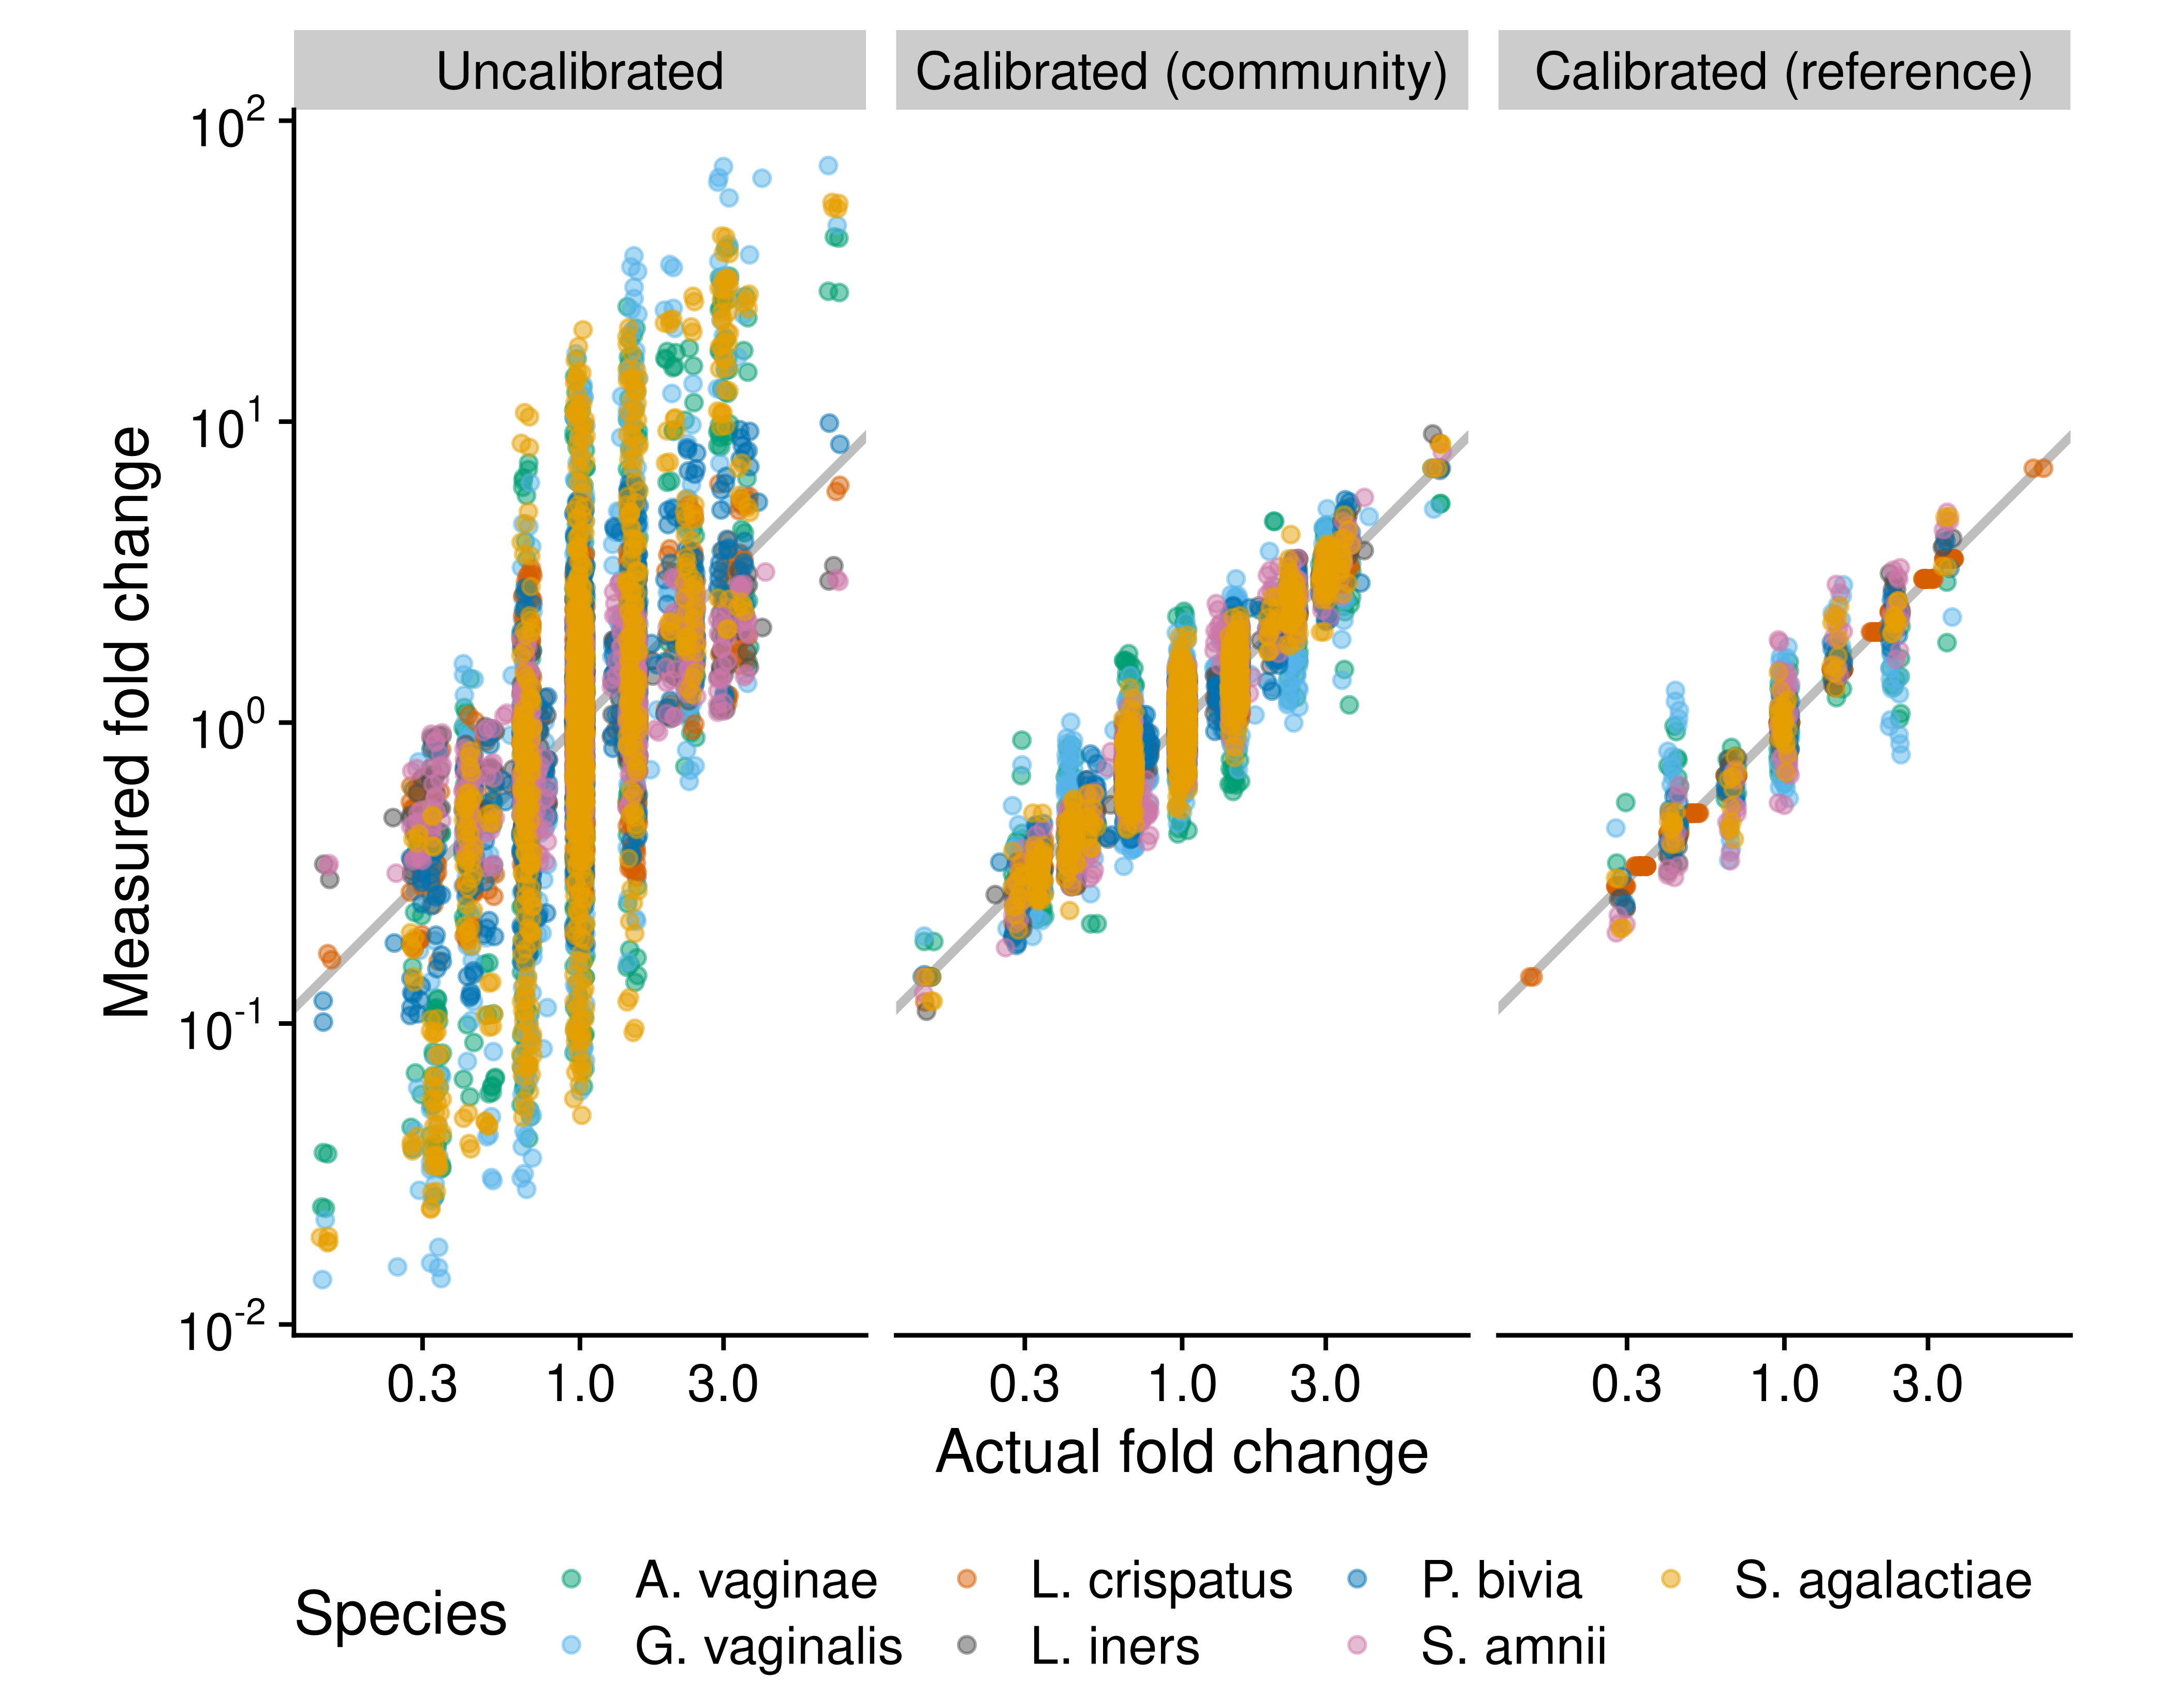
\includegraphics[width=1\linewidth]{notebook/_posts/2021-10-25-brooks2015thet-calibration/brooks2015thet-calibration_files/figure-html5/brooks2015thet_fc_calibration-1} \caption{\textbf{Fold changes can be calibrated using community controls or reference species.} The figure compares the performance of three methods for measuring fold changes in absolute cell density in cellular mock communities of 7 vaginal species, which were constructed and measured via 16S sequencing by Brooks et al. (\protect\hyperlink{ref-brooks2015thet}{2015}). The `Uncalibrated' fold changes are derived directly from uncalibrated individual abundance measurements, which equal the product of the species' proportion by the total density (which here is be known to be constant by construction). The `Calibrated (community)' measurements are computed from abundance measurements where the proportions are first corrected for the taxonomic bias that was estimated from a single sample that contained all 7 species. The `Calibrated (reference)' measurements are computed from abundances measured with the reference-species method, with \emph{Lactobacillus crispatus} used as the reference; that is, the true abundance of \emph{L. crispatus} is treated as known and used to infer the abundance of the remaining 6 species. Only samples that contain \emph{L. crispatus} are included.}\label{fig:calibration-example}
\end{figure}



\hypertarget{calibration-using-reference-species}{%
\subsection{Calibration using reference species}\label{calibration-using-reference-species}}

Obtaining control communities that span the taxa of interest is often not practical.
Moreover, the bias that is measured from controls may differ from that in the primary samples due to differences in cell state or sample preparation.
These problems may be overcome for the purpose of species-level absolute DA analysis by using the reference-species approach to absolute-abundance measurement that was described in Section \ref{differential-abundance}.
This \emph{reference-species calibration} allows one to simultaneously account for changes in total density and the sample mean efficiency, obtaining accurate fold changes in absolute density from taxonomically biased, relative metagenomics measurements.

To demonstrate the ability for reference calibration to improve fold changes, we treated the abundance of one species (\emph{Lactobacillus crispatus}) in the Brooks et al. (\protect\hyperlink{ref-brooks2015thet}{2015}) mock community data as known, and used it to calibrate the abundances of all species.
Doing so improved the resulting measurements of fold changes in density for all species (Figure \ref{fig:calibration-example}).

Two categories of reference species have so far been used: Housekeeping species assumed to have constant abundance and spike-in species added at known (and typically constant) abundance.
The implications of bias for these methods hadn't been previously investigated.
Our results show that, provided that taxonomic bias among all species (including the housekeeping or spike-in species) is consistent across samples, then the fold error in species abundances is constant and does not impact DA analysis of log- or rank-transformed species abundances.
These methods have downsides: Housekeeping species are not always available/known, and spike-ins have the downside of needing to determine species not present in the samples and an appropriate concentration in which to add them so that they form a moderate fraction of reads across samples with potentially widely varying produce of mean efficiency and total abundance.

Section \ref{abundance-measurement} presents an additional type of reference species: naturally-occurring species whose abundance has been directly measured.
For most natural ecosystems, there is unlikely to be a single species or genus that is found in all samples.
Sample coverage can be increased by measuring multiple species with complementary presence-absence patterns (Appendix {[}TODO{]}).
Coverage can also be increased by using higher-order taxa as references---for example, performing qPCR measurements targeted to a particular family rather than a particular species.
Higher-order taxa necessarily have higher prevalence than species, though may be more prone to errors from a varying efficiency across samples.
Targeted measurements of taxa that only span a subset of samples can still provide useful validation for methods.

Housekeeping taxa and spike-ins have also been used to measure changes in total-community abundance.
Our results show that the bias invariance does not apply for this purpose---the measured fold change in total abundance have an error equal to the inverse change in the sample mean efficiency.
A similar problem arises when attempting to infer changes in abundance of any higher-order taxon, unless measurement efficiency is conserved among its species.

\hypertarget{choosing-complementary-total-density-and-metagenomics-measurements}{%
\subsection{Choosing complementary total-density and metagenomics measurements}\label{choosing-complementary-total-density-and-metagenomics-measurements}}

A variety of methods for measuring total community density have been paired with either amplicon or shotgun sequencing data for the purpose of conducting absolute DA analysis using the total-density approach described in Section \ref{differential-abundance}.
Each of these methods is subject to its own taxonomic bias: Cells from different species are likely to contribute more or less efficiently to the total abundance measurement.
Consider the popular method of assessing bacterial abundance with total-16S qPCR measurement.
Even an ideal qPCR protocol that perfectly amplifies all species remains a biased measurement of cell density, since the total 16S copies in the extracted DNA contributed by each species will be proportional to its (species-specific) lysis efficiency and 16S copy-number.
Empirical evidence supports this, as qPCR measurements of total 16S copies are rarely equivalent to total cell counts, even when multiple copy numbers are taken into account ()Lloyd et al. (\protect\hyperlink{ref-lloyd2013meta}{2013})).
16S qPCR is commonly paired with 16S amplicon sequencing, with which these sources of bias are shared, perhaps along with variation in primer binding and amplification efficiency.
Methods like flow cytometry that directly measure cell density lack these biases but likely have their own that are more likely to be orthogonal to the 16S sequencing measurement.
By extending the analysis of Section \ref{differential-abundance} to include consistent taxonomic bias in the total-density measurement, we find that pairings of total-density and sequencing measurements that share large sources of taxonomic bias can lead to an offsetting of errors that reduces the error in fold-change measurement and DA inference (Appendix \ref{total-density-bias}).
This finding suggests that methods of total-density measurement that are more accurate as measures of total cell density may actually perform worse than less accurate methods for the purposes of absolute DA inference.

We illustrate with a hypothetical example of two vaginal communities of equal density, but which are dominated either by \emph{Lactobacillus iners} or \emph{Gardnerella vaginalis}.
Based on our earlier analysis in McLaren, Willis, and Callahan (\protect\hyperlink{ref-mclaren2019cons}{2019}), we estimate that \emph{L. iners} yields 10X more 16S copies per cell than \emph{G. vaginalis} in extracted DNA.
Ignoring other sources of bias, we expect relative efficiencies of \emph{L. iners}:\emph{G. vaginalis} of 10 for both qPCR and 16S sequencing measurements.
Consequently, the \emph{G. vaginalis} community will yield a substantially lower qPCR measurement than the \emph{L. iners} community and we would incorrectly infer a decrease in total abundance.
At the same time, this decrease in the mean efficiency of the sequencing measurement would cause artificially high fold changes in the proportions of all species (Section \ref{differential-abundance}).
When using qPCR and 16S sequencing measurements for community-based density estimation, these two opposing errors cancel, yielding accurate fold changes in species densities.

More generally, changes in the mean efficiency of the total-density measurement can offset those in the sequencing measurement when comparing log density of species across samples.
If the (log) efficiencies of the total and sequencing measurement are positively correlated across species, then the (log) mean efficiencies will tend to be positively correlated across samples, leading to a reduction in error in DA analysis relative to total-density methods whose efficiencies are uncorrelated with those of the sequencing measurement.
These observations suggest that qPCR of a marker gene may be the ideal pairing for amplicon sequencing measurements, despite being a poor measure of changes in total cell density.
Similarly, bulk DNA quantification may be an ideal pairing for shotgun sequencing, making it possible to account for variation in lysis efficiency and genome length.
These pairings even make it possible to account for error caused by variation among samples in the fraction of unclassified reads, which can form a major fraction of amplicon and shotgun data.
Importantly, maximizing the offsetting of errors requires thoughtful choices during bioinformatic analysis, perhaps eschewing the filtering and normalization steps used in many software packages and workflows (Appendix \ref{total-density-bias}).

\hypertarget{bias-sensitivity-analysis}{%
\subsection{Bias-sensitivity analysis}\label{bias-sensitivity-analysis}}

For experiments that have been conducted without calibration controls, it is still possible to investigate the likelihood that DA results can be explained by taxonomic bias by performing a computational bias-sensitivity analysis.

A bias-sensitivity analysis examines how sensitive the results of a given DA analysis are to the working assumption about the bias of a given protocol.
This working assumption is typically is that there is no bias, but could also be bias measured in a previous experiment or predicted from taxonomic features like 16S copy number.
A straightforward approach to bias-sensitivity analysis is to use computer simulation to re-analyze the MGS data across a set of simulated taxonomic biases.
First, multiple sets of efficiency vectors are randomly generated, each representing a possible quantification of taxonomic bias for the study.
Second, each efficiency vector is used to calibrate the original MGS measurements; each set of calibrated measurements represents the true community compositions under the given hypothesized bias.
Finally, the DA analysis is re-run on each set of calibrated measurements and the distribution of results is compared graphically or with summary statistics.
A graphical summary of such an analysis being applied to results from the corncob frequentist DA- analysis tool `corncob' are shown in SI Figure \ref{fig:sensitivity-example}.
The simulated efficiency vectors may be generated to different hypotheses about bias in the given system, such as its overall magnitude and correlation among phylogenetically-related species.
Thus the utility of such simulations will increase the more we learn about the properties of taxonomic bias in different systems.

An alternative approach to bias-sensitivity analysis would be to directly include the (unknown) taxonomic bias of the protocol in the statistical model used for DA analysis, as described for bias-aware meta-analysis below.
Further development of tools and workflows for performing bias sensitivity analyses could be a valuable way to assay and improve the reliability of microbiome results---for differential abundance and microbiome analyses more generally.

\hypertarget{bias-aware-meta-analysis}{%
\subsection{Bias-aware meta-analysis}\label{bias-aware-meta-analysis}}

So far we have considered analysis of samples subject to the same taxonomic bias;
however, meta-analysis of microbiome samples measured across multiple studies must often contend with a diversity of protocols and hence taxonomic biases in samples from different studies.
This inconsistency in taxonomic bias across studies poses a problem even for ratio-based analyses.
A potential solution is to perform a bias-aware meta-analysis that that explicitly accounts for the possibility of distinct taxonomic bias across studies.

Parametric microbiome meta-analysis models include sets of species-specific latent parameters to model ``batch effects''---amorphous differences in the measurements of each study.
By configuring these models so that these latent parameters correspond to study-specific species efficiencies, we can improve their biological interpretability and gain the ability to directly assess whether disagreements in DA results across studies can be explained by differences in taxonomic bias.
To the extent that taxonomic bias truly is consistent within studies, meta-analyses that directly account for it can have greater statistical power to extract the truly consistent and inconsistent microbial patterns across studies.

\hypertarget{todo-summary}{%
\subsection{{[}TODO{]} Summary}\label{todo-summary}}

\hypertarget{conclusion}{%
\section{Conclusion}\label{conclusion}}

It is commonly thought that analyses of the differences between samples are robust to the taxonomic bias inherent in MGS measurement as long as all samples have been subjected to the same MGS workflow.
But our results show that consistent taxonomic bias is still capable of creating scientific errors in common forms of DA analysis.
In particular, we showed mathematically that bias affects DA analysis methods based on proportions or in absolute abundances derived from them (using total-abundance normalization), due to variation in the mean efficiency across samples of varying taxonomic composition.
The error, however, varies by experimental context and may often be negligible in a practical sense.
Moreover, it can be quantified and corrected through the use of reference-taxon measurements and/or community calibration controls.
In addition, bias-aware sensitivity and meta-analyses make it possible to rigorously account for bias even in the absence of such controls.
Applications of these methods will gradually improve our understanding of the experimental contexts in which variation in the mean efficiency is likely to be problematic and should be accounted for.

We also showed that other DA methods are more robust---perhaps even entirely invariant---to consistent taxonomic bias.
In particular, analyses based on multiplicative variation in ratios and of absolute abundances derived from them (using reference-species normalization) are invariant to bias in the MGS measurement, as bias causes a constant multiplicative error that cancels in cross-sample comparisons.
In addition, careful pairing of total-abundance and MGS measurement methods may remove most of the bias-driven error in absolute abundances from total-abundance normalization.

Important open questions and future research directions remain.
Key open questions include 1) determining the extent to which bias is consistent across samples at the species level for a given MGS method and sample type; 2) assessing the validity of post-extraction absolute-abundance controls as measures of pre-extraction abundance; 3) understanding how the multiplicative error from bias interacts with the non-multiplicative error from contamination and taxonomic misassignment; and 4) understanding how our assumptions about underlying community dynamics, and in particular what information zero counts provide, affect bias sensitivity.
In addition, while we have showed some simple methods for incorporating bias and control measurements into DA analyses, better statistical tools are needed that are capable of including taxonomic bias and uncertainty in the MGS and supplemental non-MGS measurements.
Finally, more concrete experimental recommendations and user-friendly statistical workflows are needed for implementing the solutions we propose in various experimental contexts.

Our theoretical framework and example analyses provide a foundation for addressing these open questions and developing a practical experimental protocols and statistical tools.
We look to a future in which microbiome researchers routinely choose an appropriate combination of experimental and data-analytic methods capable of answering their fundamental question while accounting for taxonomic bias and the other inherent limitations of MGS measurements---and in this way, gaining the confidence needed to codify statistical findings into true scientific knowledge.

\hypertarget{appendix-appendix}{%
\appendix \addcontentsline{toc}{section}{\appendixname}}


\hypertarget{model-details}{%
\section{Model details}\label{model-details}}

This appendix provides a more detailed description of our deterministic model of the microbiome measurement process, which it uses to derive some of the additional claims of the main text.

\hypertarget{mgs-measurement}{%
\subsection{MGS measurement}\label{mgs-measurement}}

This section expands the description of the model in the main text to more explicitly lay out our assumptions and to consider the effect of variation in measurement efficiencies within a taxonomic group on its MGS measurement.

A taxon can be any group of organisms.
For any taxon \(I\) and sample \(a\), we define the absolute efficiency of that taxon and that sample as the number of reads assigned to that taxon divided by the number of cells of that taxon in the given sample.
We assume that these assigned reads really do come from that particular taxon and sample (though this assumption is often violated in practice).

The efficiency of a taxon \(I\) is the average number of reads produced by each of its constituent cells.
This number varies due to

\begin{enumerate}
\def\labelenumi{\arabic{enumi}.}
\tightlist
\item
  Genetic variation among cells
\item
  Non-genetic variation among cells
\item
  Randomness in the experimental process
\end{enumerate}

Variation encoded in the genome of cells determines properties that affect its efficiency, such as how easy it is to lyse, how easily PCR primers will bind to their target locus, how many copies of a marker gene are in the genome, and whether its sequencing reads can be taxonomically assigned.
This variation created by genetically encoded traits is what we refer to as `taxonomic bias' and is the primary focus of this article.
In principle, even a single nucleotide change (e.g.~in a primer-binding site) could affect the efficiency of a cell.
Nevertheless, cells will more similar genomes will tend to have more similar genetically-encoded efficiencies.
For the purposes of our analysis, we suppose that cells within the same species have approximately identical genetically-encoded efficiencies.
The impact of violations in this assumption can be understood using the approach we describe below for taxa above the species level.
More generally, our results can be read as applying to the finest taxonomic unit that is reported by the given MGS method.

Genetically identical cells can differ in cell state such that their efficiencies vary significantly.
An extreme example is the effect of sporulation: Spores are generally harder to lyse than vegetative cells, and VanInsberghe et al. (\protect\hyperlink{ref-vaninsberghe2020diar}{2020}) found that the efficiency of a common DNA extraction protocol was 800X on vegetative cells vs spores of a strain of \emph{Clostridium difficile}.
Physiological differences might also arise simply due where they are in the cell cycle.
To the extent that the cells of a given genotype tend to have a similar distribution of cell states across samples, the efficiency of the genotype will remain stable.
We assume this stability throughout our analysis.
Violations in this assumption can again be understood using an approach similar to that we use to considering taxa above the species level.

The final number of reads also varies due to idiosyncratic events that we typically think of (and model) as `random', such as the precise handling of a sample during pipetting or loading of a sequencing flow cell.
Such variation may or may not be dwarfed by the `random' variation in the sample composition (i.e., the variation not explained by the covariates in a regression analysis).
For simplicity, we ignore this random variation when considering the impact of taxonomic bias on MGS measurement.
The effect of random variation in regression analysis is addressed in Appendix \ref{appendix-regression} and the effect of random counting error is discussed in Section \ref{case-studies}.

The absolute efficiency of a taxon can also vary simply because more effort is put towards sequencing that sample, either intentionally or unintentionally.
The sequencing effort might depend on the taxonomic composition and bias of a sample.
For example, a sample with higher output DNA will often be diluted more prior to amplification or sequencing.
The critical assumption we make regarding sequencing effort is that it affects all species in the sample equally and hence doesn't affect their relative abundances.

With these assumptions in place, we can partition the multiplicative difference between the reads assigned to a taxon and its density in the source sample into a taxon-specific factor and a sample-specific factor.
There is an extra degree of freedom, which we settle by equating the taxon-specific factors with relative measurement efficiencies and arbitrarily choose the relative efficiency of a particular species to equal 1.

Our model for the read counts of a species \(i\) in sample \(a\) can thus be expressed mathematically as
\begin{align}
  \text{reads}_{i}(a)
  = \text{density}_{i}(a) \cdot \text{efficiency}_{i} \cdot \text{effort}(a).
\end{align}
Note that the species' efficiencies are properties of the species \(i\) but not the sample \(a\).
Similarly, let \(\text{density}_{I}(a)\), \(\text{reads}_{I}(a)\), and \(\text{efficiency}_{I}(a)\) denote the density, read count, and relative efficiency of an arbitrary group of species \(I\) in sample \(a\).
The read count for taxon \(I\) in sample \(a\) can be written
\begin{align}
  \label{eq:measurement-model-general}
  \text{reads}_{I}(a)
  = \text{density}_{I}(a) \cdot \text{efficiency}_{I}(a) \cdot \text{effort}(a).
\end{align}
The efficiency of taxon \(I\) in sample \(a\) equals the weighted average of its constituent species,
\begin{align}
  \label{eq:efficiency-general}
  \text{efficiency}_I(a) 
  \equiv \frac{\sum_{i\in I}\text{density}_i(a)\cdot \text{efficiency}_i}{\text{density}_I(a)}.
\end{align}
The ratio between the read counts of two taxa \(I\) and \(J\) is
\begin{align}
  \label{eq:ratio-error-general}
  \widehat{\text{ratio}}_{I/J}(a)
  &= \frac{\text{density}_{I}(a)}{\text{density}_{J}(a)} \cdot \frac{\text{efficiency}_{I}(a)}{\text{efficiency}_{J}(a)}.
\end{align}
Equation \eqref{eq:prop-error} for the error in a species' proportion and Equation \eqref{eq:ratio-error} for the error in the ratio between two species both follow directly from this more general expression.

\hypertarget{total-density-bias}{%
\subsection{Taxonomic bias in total-density measurement}\label{total-density-bias}}

To understand the impact of taxonomic bias in the total-density measurement on community normalization, we model error in total-density measurements similarly to that for MGS measurements.
Let \(\widehat{\text{density}}_{S}(a)\) be the measurement of the density of all species \(S\).
We suppose that this number is the sum of the (unobserved) contributions from each species.
The contribution of a species \(i\) is proportional to its actual density \(\text{density}_{i}(a)\) and its \emph{absolute efficiency for the total-density measurement} \(\text{efficiency}_{i}^{\text{tot}}(a)\).
The contributions may also be multiplied by a common sample-specific error factor to account for non-linearity of extraction and/or random error, which we ignore for now.
The measured total density therefore equals
\begin{align}
  \widehat{\text{density}}_S(a) 
  &= \sum_{i\in S} \text{density}_i(a) \cdot \text{efficiency}^{\text{tot}}_i
\\&= \text{density}_S(a) \cdot \text{efficiency}^{\text{tot}}_S(a)
\end{align}
where
\begin{align}
  \label{eq:app-total-mean-efficiency}
  \text{efficiency}^{\text{tot}}_S(a) 
  \equiv \frac{\sum_{i \in S}\text{density}_j(a)\cdot \text{efficiency}^{\text{tot}}_i}{\text{density}_S(a)}
\end{align}
is the mean efficiency in the sample with respect to the total-density measurement.

The error in the total density depends on the species composition through the mean efficiency of the sample; hence spurious changes in measured density can occur simply due to shifts from high- to low-efficiency species (or vice versa).

How does this error affect the measured densities of individual species when the total is used for normalization?
Substituting the mean efficiency of the total measurement for the error term in Equation \eqref{eq:density-prop-error} gives
\begin{align}
  \label{eq:density-prop-error-with-total-error}
  \widehat{\text{density}}_{i}(a) 
  = \text{density}_{i}(a) \cdot \frac{\text{efficiency}_{i} \cdot \text{efficiency}^{\text{tot}}_S(a)}{\text{efficiency}_S(a)}.
\end{align}
The mean efficiency of the total measurement appears in the numerator, while the mean efficiency of the MGS measurement is in the denominator.
To the extent that these two are positively associated across samples (specifically, their logarithms are positively linearly correlated), then the variation in one will tend to be offset by the variation in the other.
In this case the (geometric) variation in the ratio will be reduced, and the fold error in the species density measurement will tend to be more consistent than if the total density measurement was taxonomically unbiased (i.e.~\(\text{efficiency}^\text{tot}_S(a) = 1\) for all samples).
The error in species densities for individual samples may not be reduced; but the error in fold changes and regression analysis across samples will be.

The extent to which the log mean efficiency of the MGS measurement and the total measurement are correlated depends on the species efficiencies as well as the changes in species composition across samples, making it difficult to make general statements about this effect.
We can get a sense for the effect by considering the correlation between log efficiencies across species between the two measurement types.
Suppose that distribution over species of log efficiencies of the MGS measurement has variance \(\sigma^{2}\), the log efficiencies for the total density measurement has variance \(\sigma_{\text{tot}}^{2}\), and the correlation between the two is \(\rho\).
The variance in the difference \(\log \text{efficiency}_{i}^{\text{tot}} - \log \text{efficiency}_{i}\) is thus \(\sigma^{2} + \sigma_{\text{tot}}^{2} - \rho \sigma \sigma_{\text{tot}}\).
All else equal, the smaller this variance, the smaller we expect the variation in the error factor \(\text{efficiency}^{\text{tot}}_S(a)/ \text{efficiency}_S(a)\).

\textbf{Unclassified reads:} It is common that a given MGS protocol generates sequencing reads from particular taxa that the bioinformatics portion entirely discards, due to an inability to taxonomically assign the reads to the chosen taxonomic units.
For instance, 16S data that is analyzed with closed-reference OTU assignment and shotgun data analyzed by mapping to a database of reference genomes will be unable to assign sequences that are less than a chosen similarity cutoff (e.g.~97\%) from the reference sequences.
These taxa may form an appreciable fraction of the community and thus lead to a large fraction of the total sequenced reads for a given sample may remain unassigned.

So far, we have defined the efficiency of the MGS protocol in terms of taxonomically classified reads and so have treated such taxa as having an MGS efficiency of 0.
If such species are included in the total density measurement, then we have a mismatch between the two measurement types.
However, we may be able to remove this mismatch by altering the equation we use to form species density measurements.
In particular, we can compute the proportion of the focal species from the ratio of its assigned reads to the total sequenced reads, rather than to the total set of assigned reads.
This approach raises additional questions around how to treat reads from assignable species that are filtered during quality control steps.

Suppose that the set of species that can be classified by our bioinformatics pipeline, \(S\), is a proper subset of a larger set of species \(S'\) that are present and yield sequencing reads in our sample.
Suppose that there is no additional taxonomic bias in our MGS measurement; that is, all species in \(S\) have an efficiency of 1, and the species in \(S' \setminus S\) have an efficiency of 0.
Moreover, suppose that all reads from the \(S\) species are classified; that is, there is no loss of reads due to routine QC filtering.
Further suppose that we are capable of perfectly measuring the total density of all cells from the full set of species \(S'\); that is, \(\text{efficiency}^{\text{tot}}_{i} = 1\) for all species \(i \in S'\).

In this case, we can overcome the mismatch between MGS and total measurement when we use them to measure species densities, by using the total reads rather than the assigned reads to compute the species proportions.
That is, instead of
\begin{align}
  \widehat{\text{prop}}_{i}(a) = \frac{\text{reads}_i(a)}{\text{reads}_S(a)},
\end{align}
we take
\begin{align}
  \widehat{\text{prop}}_{i}(a) 
  &= \frac{\text{reads}_i(a)}{\text{total reads}(a)}
\\&= \frac{\text{reads}_i(a)}{\text{reads}_{S'}(a)}.
\end{align}
By accounting for the contribution of unknown species when computing proportions, we are able to resolve the mismatch and obtain accurate species densities.

\hypertarget{total-density-ref}{%
\subsection{Using reference species for total-density normalization}\label{total-density-ref}}

Constant reference species are sometimes used to measure total density of \(S\) by the ratio of \(S\) reads to \(R\) reads.
For example, a study of \emph{Arabidopsis} microbiomes used the ratio of bacterial to host reads in shotgun sequencing as a proxy for total bacterial density, which they then used for total-community normalization of 16S amplicon sequencing measurements (Karasov et al. (\protect\hyperlink{ref-karasov2020ther}{2020}), Regalado et al. (\protect\hyperlink{ref-regalado2019comb}{2020})).
Chng et al. (\protect\hyperlink{ref-chng2020meta}{2020}) similarly used the ratio of bacterial to host or diet reads in shotgun sequencing of mouse fecal samples as a proxy for total bacterial density (though they did not use this measurement for community normalization).
Smets et al. (\protect\hyperlink{ref-smets2016amet}{2016}) similarly used the ratio of non-spike-in to spike-in reads to estimate total density.

What is the impact of taxonomic bias on these total density estimates and the species densities derived from them?
The measured density of \(S\) is
\begin{align}
  \widehat{\text{density}}_{S}(a) 
  &= \frac{\text{reads}_S(a)}{\text{reads}_{R}(a)}
\\&= \frac{\text{density}_S(a)}{\text{density}_{R}} \cdot \frac{\text{efficiency}_S(a)}{\text{efficiency}_{R}}
\\&= \text{density}_S(a) \cdot \text{efficiency}_S(a) \cdot \text{constant}.
\end{align}
Hence variation in the mean efficiency among the species \(S\) across samples creates a variable fold error in the density measurement, similar to direct measurements of total density.

The impact of this variable error for species density measurement via Equation \eqref{eq:density-prop-meas} depends on whether the species proportions are derived from the same or a different MGS measurement.

If proportions from the same MGS measurement are used, then the measured species densities are
\begin{align}
  \widehat{\text{density}}_{i}(a) 
  &= \frac{\text{reads}_i(a)}{\text{reads}_{S}(a)} \cdot \widehat{\text{density}}_{S}(a)
\\&= \frac{\text{reads}_{i}(a)}{\text{reads}_{R}(a)}.
\end{align}
where the second line follows by substitution of the previous equation.
The variable error in the total density cancels with that in the proportion, yielding a constant fold error.
In fact, the measurement we obtain is exactly the same as that from reference normalization (Equation \eqref{eq:density-ratio-meas}).

The situation differs when the total density and community composition are estimated using different sequencing and/or bioinformatic methods, as in the plant microbiome example above.
In this case, the mean efficiency of the total density measurement will not equal that in the proportions, and the more general case of total-density normalization discussed in Appendix \ref{total-density-bias} applies.

Although we only consider constant reference species, similar behavior occurs if for varying reference species assayed by targeted measurements.

\hypertarget{linearity-of-extraction}{%
\subsection{Linearity of extraction}\label{linearity-of-extraction}}

Some popular absolute-abundance methods use post-extraction DNA (or RNA) density as a proxy for cell density in the original sample; in particular, using florescence-based total DNA quantification or using qPCR or ddPCR to quantify a marker-gene.
In addition, some have suggested normalization of species to spike-ins of extraneous DNA added after extraction.
Both of these approaches presuppose that DNA extraction is linear in the sense that the DNA concentration is proportional to the cell concentration in the original sample (possibly after correction by known dilution or concentration factors).
Deviations from linearity can occur due to random and systematic variation in DNA yields.
Here we consider the impact of these deviations on species density measurements.

One source of systematic variation in yield is taxonomic bias.
We already explored the impact of taxonomic bias in extraction.

NOTE: This might not be a correct way to talk about this; should perhaps make a more explicit model to verify this argument.

To understand the impact of non-linearity after bias has been accounted for, let \(C(a)\) be a sample-specific factor that accounts for DNA extraction non-linearity after controlling for bias.
From Equation \eqref{eq:density-prop-error}, we have the more general equation
\begin{align}
  \label{eq:density-prop-error-linearity}
  \widehat{\text{density}}_{i}(a) 
  = \text{density}_{i}(a) \cdot \frac{\text{efficiency}_{i} \cdot \text{efficiency}^{\text{tot}}_S(a)}{\text{efficiency}_S(a)} \cdot C(a).
\end{align}
\(C(a)\) might fluctuate randomly among samples, or might vary systematically --- for example, if DNA yield saturates at high concentrations then \(C(a)\) will be smaller in higher-concentration samples.
If DNA extraction is not linear, then measures of cell density might give more accurate fold changes even if they share less bias with the MGS measurement.

Post-extraction spike-ins and targeted measurements face a similar problem.
These perfectly control for bias in fold change estimation \emph{if} DNA extraction is linear.
However, if not then the fold error in \(\widehat{\text{density}_r}(a)\) for a species with a targeted measurement will vary with \(C(a)\) and cause error in fold changes.
The same problem applies to DNA spike-ins added after DNA extraction (although different accounting is needed since \(\text{density}_r(a)\) no longer has meaning).

\hypertarget{review-absolute-methods}{%
\section{Review of experimental methods for obtaining absolute densities}\label{review-absolute-methods}}

There are many experimental techniques to be able to add absolute-density information to MGS measurements.
Here we review the experimental techniques; the next section considers the implications for systematic error.

\emph{NOTE: Right now I don't consistently address why various targeted methods might be expected to produce constant fold errors. In revision, seek to connect each method with the relevant theory.}

\hypertarget{measurement-of-total-cell-density}{%
\subsection{Measurement of total cell density}\label{measurement-of-total-cell-density}}

Total cell density in the original sample can be directly measured by cell counting, either via microscopy (Kevorkian et al. (\protect\hyperlink{ref-kevorkian2018esti}{2018}), Lloyd et al. (\protect\hyperlink{ref-lloyd2020evid}{2020})) or flow cytometry (Props et al. (\protect\hyperlink{ref-props2017abso}{2017}), Vandeputte et al. (\protect\hyperlink{ref-vandeputte2017quan}{2017})).
Total cell density or biomass can also be measured via properties assumed to be proportional to cell density, such as fluorescence (as in fluorescence spectroscopy, Wang et al. (\protect\hyperlink{ref-wang2021curr}{2021})), components of microbial cell membranes (as in PLFA analysis, Smets et al. (\protect\hyperlink{ref-smets2016amet}{2016})), and the rate of microbial respiration (as in SIR method, Smets et al. (\protect\hyperlink{ref-smets2016amet}{2016})).
So far, it is primarily the cell counting methods that have been used for species-density measurement (rather than simply for the total density), by multiplying the estimated total density by the MGS proportions.

\hypertarget{measurement-of-total-dna-density-post-extraction}{%
\subsection{Measurement of total DNA density post extraction}\label{measurement-of-total-dna-density-post-extraction}}

It is also common to use density of bulk DNA or a marker gene as a proxy for total community density.
Marker-gene density is typically measured with qPCR or ddPCR using `universal primers' that target the marker gene of interest (typically the 16S gene for bacterial microbiome experiments) (Tettamanti Boshier et al. (\protect\hyperlink{ref-tettamantiboshier2020comp}{2020}), Jian et al. (\protect\hyperlink{ref-jian2020quan}{2020}), Galazzo et al. (\protect\hyperlink{ref-galazzo2020howt}{2020})).
Bulk DNA density can be measured using fluorescence-based DNA quantification assays (Contijoch et al. (\protect\hyperlink{ref-contijoch2019gutm}{2019}); Korpela et al. (\protect\hyperlink{ref-korpela2018inte}{2018})).
In either case, the DNA density is measured after DNA extraction and so is affected by taxonomic bias in the extraction process, such as variation in lysis efficiency among species.
Other sources of bias that affect the DNA density measurement include variation in marker-gene copy number (for marker-gene density) and variation in genome size (for bulk DNA density).

The measured DNA density is typically used as a direct proxy for cell density in the original sample.
In particular, it is assumed that a doubling of cell density in the original sample leads to a doubling of DNA density in the extraction (possibly after adjustment for known dilution factors).
This \emph{linearity assumption} may be violated for several reasons.
First, because of taxonomic bias.
For example, samples dominated by easy-to-lyse species will give more DNA per cell than samples dominated by hard-to-lyse species.
Second, systematic non-linearity may occur in the DNA yield as a function of input, even if species composition is held fixed.
For example, DNA yield may saturate at high sample inputs.
Third, the DNA yield may vary apparently randomly due to subtle differences in sample chemistry or handling during the experiment.

\hypertarget{equivolumetric-protocol}{%
\subsection{Equivolumetric protocol}\label{equivolumetric-protocol}}

A large part of the reason that there is not a direct correspondence between total density in the sample and total reads sequenced is that MGS experiments are typically intentionally designed to yield a similar number of sequencing reads from each sample, regardless of total density.
Cruz, Christoff, and Oliveira (\protect\hyperlink{ref-cruz2021equi}{2021}) propose instead designing the MGS experiment so as to make total reads proportional total density.
The `equivolumetric protocol' they develop represents a first attempt in this direction.
In their protocol, total reads is a saturating function of total density; this function can be measured with a calibration experiment, and the calibration curve used to predict the total density in the source sample.
This total density estimate is then used to scale the read counts to estimate species densities in a manner equivalent to the total-community density method.

\hypertarget{housekeeping-species}{%
\subsection{Housekeeping species}\label{housekeeping-species}}

We use \emph{housekeeping species} (by analogy with housekeeping genes used for normalization in RNAseq experiments) to refer to species whose density is assumed to be constant, either in the MGS sample or in the source ecosystem it is derived from.

Housekeeping species can sometimes be identified from prior scientific knowledge.
Several studies that have employed shotgun sequencing of host-associated microbiomes have use the plant or animal host for this purpose.
A study of \emph{Arabidopsis} microbiomes used the ratio of bacterial to host reads in shotgun sequencing as a proxy for total bacterial density, which they then used for total-community normalization of 16S amplicon sequencing measurements (Karasov et al. (\protect\hyperlink{ref-karasov2020ther}{2020}), Regalado et al. (\protect\hyperlink{ref-regalado2019comb}{2020})).
Chng et al. (\protect\hyperlink{ref-chng2020meta}{2020}) similarly used the ratio of bacterial to host reads in shotgun sequencing of mouse fecal samples as a proxy for total bacterial density (though they did not use this measurement for community normalization).
They also use reads from dietary plants for the same purpose.
Wallace et al. (\protect\hyperlink{ref-wallace2021thed}{2021}) used shotgun sequencing to study the virome of \emph{Drosophila}, and normalized virus reads to \emph{Drosophila} reads to measure viral abundance per fly.
Organelle reads can also be used.
Diener et al. (\protect\hyperlink{ref-diener2021nonr}{2021}) use mitochondria reads in 16S sequencing of mouse fecal pellets to assess total microbial load, though in a qualitative fashion (as mitochondrial reads were only non-zero at very low bacterial densities induced by antibiotics).

In some cases, there may also be microbes or viruses thought to have stable densities.
A recent example is that the most abundant DNA virus in human feces, crAssphage, and the most abundant RNA virus in human feces, Pepper Mild Mottle Virus, have been treated as stable reference species in wastewater monitoring for SARS-CoV-2.
Although primarily used in the context of qPCR measurements, these viruses could also be used as references in RNA and DNA shotgun sequencing experiments.

Housekeeping species may not be known \emph{a priori}; to address this case, several methods have been put forward to computationally identify unchanging microbes species directly from MGS measurements.
These studies are often focused on mammalian gut bacterial communities.
It is perhaps unreasonable to expect bacterial species to be unchanging across hosts, but weaker assumptions can be made to develop normalization methods for the MGS measurements with a similar spirit to reference-based normalization.
These studies have instead developed normalization methods based on assumptions such as that most species do not change between any pair of samples (David et al. (\protect\hyperlink{ref-david2014host}{2014})) or that the mean (log) abundance between two sample conditions is unchanged for at least some species (Mandal et al. (\protect\hyperlink{ref-mandal2015anal}{2015}), Kumar et al. (\protect\hyperlink{ref-kumar2018anal}{2018})).

When housekeeping species are sequenced along with the primary MGS measurement, they can be used to obtain species densities via reference-normalization (Equation \eqref{eq:density-ratio-meas}.
In this case, the only relevant taxonomic bias is that of the primary MGS measurement; if it is constant then it will cancel in fold-change calculations.
Because the density of the housekeeping species is unknown, we can consider either that the density of focal species has a constant error, or is in units of the housekeeping species.
Non-constant error might arise if the species is treated as constant when it is in fact not.

Housekeeping species have also been used to estimate total community density by \(\text{reads}_{S} / \text{reads}_{R}\).
This estimate has been used to study variation in total density across samples, or for total-density normalization.

\hypertarget{spike-ins}{%
\subsection{Spike-ins}\label{spike-ins}}

Spike-in methods differ by the biological spike-in material:
Cellular spike-ins can be added prior to DNA extraction, and DNA spike-ins can be added prior to or following DNA extraction.
In either case, a variety of methods can be used to actually leverage the spike-ins for absolute density analysis.

\textbf{Cellular spike-ins:}
Cellular spike-ins are added to the sample prior to DNA extraction.
Some sample processing has typically occurred prior to spiking, for the purposes of storage (e.g.~a freeze thaw cycle) and homogenization.
We should expect there to be taxonomic bias between the spike-in species and those naturally in the sample due to genetic differences and because of physiological differences induced by the sample processing prior to spiking and the experimental procedure used to grow and prepare the spike-in cells.
Our analysis acknowledges this bias, but assumes that it is consistent across samples.
The nominal density of the spike-in species added to each sample is subject to random and systematic fold error; but systematic fold error that is shared across samples will induce a constant fold error in species densities and so not impact DA analysis.
For instance, if source stock is actually 1.5X higher concentration than thought, the true spike-in concentration will be 1.5X greater than nominal in all samples and not pose a problem for accurate DA inference beyond leading to a greater than intended sequencing effort being expended on the spike-in.

Example studies include Stämmler et al. (\protect\hyperlink{ref-stammler2016adju}{2016}), Ji et al. (\protect\hyperlink{ref-ji2019quan}{2019}), and Rao et al. (\protect\hyperlink{ref-rao2021mult}{2021}).

\textbf{DNA spike-ins:}
Another possibility is to add DNA spike-ins, derived from natural or artificial sequence.
DNA spike-ins can be added the samples before DNA extraction (e.g. Smets et al. (\protect\hyperlink{ref-smets2016amet}{2016}), Tkacz, Hortala, and Poole (\protect\hyperlink{ref-tkacz2018abso}{2018}), Zemb et al. (\protect\hyperlink{ref-zemb2020abso}{2020})) or after DNA extraction (e.g. Hardwick et al. (\protect\hyperlink{ref-hardwick2018synt}{2018}), Tkacz, Hortala, and Poole (\protect\hyperlink{ref-tkacz2018abso}{2018})).
Adding spike-ins prior to extraction is thought to be preferable as it makes it possible to detect and correct for variation in DNA extraction yield among samples
(Tkacz, Hortala, and Poole (\protect\hyperlink{ref-tkacz2018abso}{2018}), Zemb et al. (\protect\hyperlink{ref-zemb2020abso}{2020}), Harrison et al. (\protect\hyperlink{ref-harrison2021theq}{2021})).
Below, we consider the distinction between pre- and post-extraction spike-ins in the light of taxonomic bias coupled with other sources of variation in extraction efficiency.

\textbf{How spike-ins are used:}
Like housekeeping species, spike-ins have been used in a variety of ways to analyze absolute abundances.
Let \(R\) (for reference) be the spike-in species and \(S\) be the native species.
Smets et al. (\protect\hyperlink{ref-smets2016amet}{2016}) used the ratio of \(S\) to \(R\) reads as an estimate of total density, which they were interested in for its own sake, though one could imagine then also using this total density estimate in community normalization (Equation \eqref{eq:density-prop-meas}).
Zemb et al. (\protect\hyperlink{ref-zemb2020abso}{2020}) used the spike-ins to measure total density from the ratio of \(S\) to \(R\) qPCR abundance estimates and then used Equation \eqref{eq:density-prop-meas}.
Stämmler et al. (\protect\hyperlink{ref-stammler2016adju}{2016}) and others used the ratio-based method of Equation \eqref{eq:density-ratio-meas}.

\hypertarget{targeted-measurements}{%
\subsection{Targeted measurements}\label{targeted-measurements}}

A variety of methods exist for targeted measurement of absolute density of a specific species (or higher-order taxon).
The most common approach is to use qPCR or ddPCR to measure the concentration of a marker gene in the extracted DNA, using primers scoped to the target taxon.
This approach is therefore subject to sources of taxonomic bias including extraction, marker-gene copy number, and primer-binding.
It is also subject to non-species-specific variation in extraction yields unless these are otherwise controlled for.
It is also possible to directly measure cell density using methods.
Some species can be measured by CFU counting after plating on selective media (REFs), and ddPCR has been used to direct measure cells (Dreo et al. (\protect\hyperlink{ref-dreo2014opti}{2014}), Morella et al. (\protect\hyperlink{ref-morella2018rapi}{2018})) and viruses (Pavšič, Žel, and Milavec (\protect\hyperlink{ref-pavsic2016digi}{2016}), Morella et al. (\protect\hyperlink{ref-morella2018rapi}{2018})) without first performing an extraction.
Species-specific florescent probes also make it possible to measure individual species via microscopy or flow cytometry (REFs).

TODO: Argue that these methods may yield constant fold errors.

\hypertarget{appendix-regression}{%
\section{Taxonomic bias and linear regression}\label{appendix-regression}}

This section derives the theoretical results of Section \ref{differential-abundance} for the effect of taxonomic bias on regression-based DA analyses.
As in Section \ref{differential-abundance}, we restrict our attention to DA analyses that can be expressed in terms of the simple linear regression model in which the response is log absolute abundance or log proportion of individual species or the log ratio of a pair of species.

\hypertarget{review-of-simple-linear-regression}{%
\subsection{Review of simple linear regression}\label{review-of-simple-linear-regression}}

\begin{longtable}[]{@{}
  >{\raggedright\arraybackslash}p{(\columnwidth - 4\tabcolsep) * \real{0.23}}
  >{\raggedright\arraybackslash}p{(\columnwidth - 4\tabcolsep) * \real{0.38}}
  >{\raggedright\arraybackslash}p{(\columnwidth - 4\tabcolsep) * \real{0.38}}@{}}
\caption{\label{tab:statistical-notation} Statistical notation used in this section.}\tabularnewline
\toprule
\begin{minipage}[b]{\linewidth}\raggedright
Notation
\end{minipage} & \begin{minipage}[b]{\linewidth}\raggedright
Mathematical definition
\end{minipage} & \begin{minipage}[b]{\linewidth}\raggedright
Description
\end{minipage} \\
\midrule
\endfirsthead
\toprule
\begin{minipage}[b]{\linewidth}\raggedright
Notation
\end{minipage} & \begin{minipage}[b]{\linewidth}\raggedright
Mathematical definition
\end{minipage} & \begin{minipage}[b]{\linewidth}\raggedright
Description
\end{minipage} \\
\midrule
\endhead
\(x\), \(y\), \(z\), \(d\) & & Random variables, defined in text \\
\(x(a)\) & & Value of \(x\) in sample \(a\) \\
\(\bar x\) & \(\frac{1}{n}\sum_a x(a)\) & Sample mean of \(x\) \\
\(s(x,y)\) & \(\frac{1}{n}\sum_a (x(a) - \bar x) (y(a) - \bar y)\) & Sample covariance between \(x\) and \(y\) \\
\(s^{2}(x)\) & \(s(x,x)\) & Sample variance of \(x\) \\
\(s(x)\) & \(\sqrt{s^{2}(x)}\) & Sample standard deviation of \(x\) \\
\(r(x,y)\) & \(\frac{s(x,y)}{s(x) s(y)}\) & Sample correlation between \(x\) and \(y\) \\
\(\alpha\), \(\beta\), \(\sigma\) & & Parameters of the regression model \\
\(\hat \alpha\), \(\hat \beta\), \(\hat \sigma\) & & Parameter estimates \\
\(\epsilon(a)\) & \(y(a) - (\alpha + \beta x(a))\) & Error for sample \(a\) \\
\(\hat \epsilon(a)\) & \(y(a) - (\hat \alpha + \hat \beta x(a))\) & Residual for sample \(a\) \\
\(\text{se}(\hat \beta)\), \(\hat{\text{se}}(\hat \beta)\) & & Standard error of \(\hat \beta\) and its estimate \\
\bottomrule
\end{longtable}

We begin by reviewing definitions, notation, and results for the analysis of the simple linear regression model.
Our presentation follows Wasserman (\protect\hyperlink{ref-wasserman2004allo}{2004}) Chapter 13 with additional interpretation of the estimated regression coefficients.
Statistical notation is defined in Table \ref{tab:statistical-notation}.

Consider a response variable \(y\) and a covariate \(x\).
Following Wasserman (\protect\hyperlink{ref-wasserman2004allo}{2004}), we define the \emph{simple linear regression model} by
\begin{align}
  \label{eq:lm}
  y(a) &= \alpha + \beta x(a) + \varepsilon(a),
\end{align}
where \(E[\varepsilon(a) \mid x(a)] = 0\) and \(V[\varepsilon(a) \mid x(a)] = \sigma^2\).
That is, conditional on the value of \(x\) in a sample \(a\), the response \(y\) is given by \(\alpha + \beta x\) with a random error \(\varepsilon\) that has an expected value of \(0\) and a constant variance \(\sigma^2\).

Given data \((y, x)\), we \emph{fit} the model by finding estimates for the parameters \(\alpha\), \(\beta\), and \(\sigma^2\) that best reflect the data under the assumption that the model is correct and according to our chosen criterion that defines `best'.
Here we consider the least-squares estimates for the coefficients \(\alpha\) and \(\beta\), which are also the maximum likelihood estimates if we further assume that the errors \(\varepsilon\) are normally distributed.
The least-squares estimates of \(\alpha\) and \(\beta\) are the values that minimize the residual sum of squares, \(\text{RSS} = \sum_{a} \hat \varepsilon(a)\).
These estimates can be conveniently expressed in terms of the sample means and covariances or correlations of \(x\) and \(y\),
\begin{align}
  \label{eq:lm-hat}
  \hat \alpha &= \bar y - \hat \beta \bar x \\
  \hat \beta &= \frac{s(y,x)}{s^2(x)} = r(y,x) \cdot \frac{s(y)}{s(x)}.
\end{align}
The estimate for the slope coefficient, \(\hat \beta\), equals the ratio of the sample covariance of \(y\) with \(x\) relative to the variance in \(x\) or, equivalently, the correlation of \(y\) with \(x\) multiplied by the ratio of their standard deviations.
The estimate for the intercept, \(\hat \alpha\), is the value such that the sample means follow the regression relationship, \(\bar y = \hat \alpha + \hat \beta \bar x\).
The standard unbiased and maximum likelihood estimates for the variance \(\sigma^{2}\) are both approximately given by the sample variance of the residuals,
\begin{align}
  \label{eq:lm-var}
  \hat{\sigma}^2(\hat \beta) \approx s^2(\hat \varepsilon).
\end{align}

We are most interested in the estimated slope coefficient, \(\hat \beta\).
Besides the point estimate indicating our best guess at the value, we also wish to understand the uncertainty or precision of the estimate.
This uncertainty is quantified by the standard error, \(\text{se}(\hat \beta)\), estimated by
\begin{align}
  \label{eq:lm-se}
  \hat{\text{se}}(\hat \beta)
  = \frac{\hat \sigma}{s(x) \sqrt{n}}
  \approx \frac{s(\hat \varepsilon)}{s(x) \sqrt{n}},
\end{align}
Approximate 95\% confidence intervals for \(\beta\) are given by \(\hat \beta \pm 2\; \hat{\text{se}}(\hat \beta)\).

\hypertarget{measurement-error-in-the-response}{%
\subsection{Measurement error in the response}\label{measurement-error-in-the-response}}

Now consider a researcher who would like to regress a biological quantity \(y\) (the response) on a second quantity \(x\) (the covariate).
But instead of \(y\), they only know a proxy \(z\), which is related to \(y\) via the difference \(d = z - y\).
For instance, \(y\) might be the log abundance of a species, \(z\) is the abundance that is measured via MGS, and \(x\) is a numerical quantity like pH or a boolean variable indicting case versus control.
Lacking a direct measurement of \(y\), the researcher instead regresses \(z\) on \(x\) and interprets the fitted model as informing them about the relationship between \(y\) and \(x\).
We wish to understand the accuracy of their conclusions.

To understand how the measurement error in \(y\) impacts the researcher's regression analysis, consider the three linear regression equations for \(y\), \(z\), and \(d\),
\begin{align}
  \label{eq:lm-y}
  y(a) &= \alpha_y + \beta_y x(a) + \varepsilon_y(a),
\end{align}
\begin{align}
  \label{eq:lm-z}
  z(a) &= \alpha_z + \beta_z x(a) + \varepsilon_z(a),
\end{align}
\begin{align}
  \label{eq:lm-d}
  d(a) &= \alpha_d + \beta_d x(a) + \varepsilon_d(a).
\end{align}
The researcher would like to fit the model for \(y\) (Equation \eqref{eq:lm-y}), but instead can only fit the model for \(z\) (Equation \eqref{eq:lm-z}).
The two are related via the Equation \eqref{eq:lm-z} for \(d\).
It is helpful to imagine, for the moment, that \(y\) and \(d\) are known and so we can fit all three models \eqref{eq:lm-y}, \eqref{eq:lm-z}, and \eqref{eq:lm-d}.
From Equation \eqref{eq:lm-hat} and the linearity of sample means and covariances it follows that
\begin{align}
  \label{eq:lm-hat-rel}
  \hat \alpha_z &= \hat \alpha_y + \hat \alpha_d \\
  \hat \beta_z &= \hat \beta_y + \hat \beta_d.
\end{align}
That is, the estimated coefficients for \(y\), \(z\), and \(d\) mirror the relationship between the variables themselves, \(z = y + d\).
Consequently, we see that the measurement error \(d\) creates absolute errors in the regression coefficients \(\hat \alpha\) and \(\hat \beta\) equal to
\begin{align}
  \label{eq:lm-hat-err}
  \text{abs. error}(\hat \alpha) &\equiv \hat \alpha_z - \hat \alpha_y = \hat \alpha_d \\
  \text{abs. error}(\hat \beta) &\equiv \hat \beta_z - \hat \beta_y = \hat \beta_d.
\end{align}
These absolute errors correspond to the \emph{statistical bias} in the coefficient estimates.
Expressed in terms of sample means and covariances, these errors are
\begin{align}
  \label{eq:lm-hat-err-1}
  \text{abs. error}(\hat \alpha) &= \bar d - \hat \beta_d \bar x \\
  \text{abs. error}(\hat \beta)  &= \frac{s(d,x)}{s^2(x)} = r(d,x) \cdot \frac{s(d)}{s(x)}.
\end{align}

We are mainly interested in the estimated slope coefficient, \(\hat \beta\).
We see that the absolute error is large when the covariance of \(d\) with \(x\) is large.
This error is large in a practical sense when \(\hat \beta_{d}\) is large (in magnitude) relative to \(\hat \beta_y\) (Equation \eqref{eq:lm-hat}), which occurs when \(s(d,x)\) is large relative to \(s(y,x)\).
A sign error occurs when \(s(d,x)\) is larger in magnitude than \(s(y,x)\) and of opposite sign.

We can also consider how the measurement error affects the residual variation and the standard error of the slope estimate.
The residuals of \(y\), \(z\), and \(d\) are related through \(\hat \varepsilon_z = \hat \varepsilon_y + \hat \varepsilon_d\).
It follows that the sample variance of the \(z\) residuals equal
\begin{align}
  s^2(\hat \varepsilon_{z}) 
  = s^2(\hat \varepsilon_y + \hat \varepsilon_{d})
  = s^2(\hat \varepsilon_y) + s^2(\hat \varepsilon_{d}) + 2 s(\hat \varepsilon_y, \hat \varepsilon_{d}).
\end{align}
The variance of the \(z\) residuals is increased above that of the \(y\) residuals when the \(d\) residuals are either uncorrelated or positively correlated with the \(y\) residuals, but may be decreased when the \(y\) and \(d\) residuals are negatively correlated.
An increased residual variance will lead to a larger estimate for \(\sigma\) as well as larger standard errors in the slope coefficient \(\beta\).

\hypertarget{specific-application-to-taxonomic-bias}{%
\subsection{Specific application to taxonomic bias}\label{specific-application-to-taxonomic-bias}}

These general results can be used to understand how taxonomic bias affects DA analyses that can be expressed as linear regression of log (relative or absolute) abundance.

First, we illustrate for the particular example of absolute DA analysis, where species absolute abundance is measured with the total-abundance normalization method and we assume that the total abundances have been accurately measured.
Consider the regression of log abundance of species \(i\) on a covariate \(x\).
In this case, \(y(a)= \log \text{abun}_{i}(a)\) is the actual log abundance of species \(i\) and \(z(a)=\log \widehat{\text{abun}}_i(a)\) is the log abundance we've measured.
From Equation \eqref{eq:density-prop-error}, the measurement error \(d(a)\) due to taxonomic bias in the MGS measurement is
\begin{align}
  d(a) 
  \equiv z(a) - y(a) 
  = \log \text{efficiency}_i - \log \text{efficiency}_S(a).
\end{align}
The absolute error in \(\hat \beta\) equals the scaled covariance of \(d\) with \(x\) (Equation \eqref{eq:lm-hat-err-1}).
In the above expression for \(d(a)\), only the second term, \(- \log \text{efficiency}_S(a)\), varies across samples and thus affects the covariance, leading to
\begin{align}
  \text{abs. error}(\hat \beta)
    &= - \frac{s[\log \text{efficiency}_S, x]}{s^2(x)}.
%    = - \frac{r[\log \text{efficiency}_S, x] \cdot s[\log \text{efficiency}_S]}{s(x)}, \\
\end{align}
Thus the absolute error in \(\hat \beta\) is the negative of the scaled covariance of the log mean efficiency.

Although the absolute error is the same for each species, its practical significance varies.
Recall from Equation \eqref{eq:lm-hat} that the correct value for \(\hat \beta\) (i.e., the estimate without measurement error) is
\begin{align}
  \hat \beta &= \frac{s[\log \text{abun}, x]}{s^2(x)}.
\end{align}
For species whose log abundance covaries with \(x\) much more than the log mean efficiency, the error will be relatively small.
This situation can occur either because the mean efficiency varies relatively little across samples or because its variation is relatively uncorrelated with \(x\).
For species whose log abundance covaries with \(x\) similar or less than the log mean efficiency, the error will be significant.
A sign error occurs when the species covariance is of \emph{equal sign and smaller in magnitude} than the covariance of the log mean efficiency.

We can also consider how the standard errors in the slope estimate are affected by bias.
In our case, the \(d\) residuals equal the negative residuals of the log mean efficiency.
It is plausible that for most species, their residual variation will have a small covariance with log mean efficiency and the net effect of variation in the mean efficiency will be to increase the estimated standard errors, as occurs with most species in Figure \ref{fig:regression-example}.
However, high-efficiency species that vary substantially in proportion across samples may be strongly positively correlated with log mean efficiency such that the estimated standard errors decrease, as we see with Species 9 in Figure \ref{fig:regression-example}.

Now, suppose we were instead performing a DA analysis of a response whose fold error is constant across samples, such as the log ratio of two species.
For the log ratio of species \(i\) and \(j\), the error is \(d(a) = \log \text{efficiency}_i / \text{efficiency}_j\) and is constant across samples.
Thus the covariance of \(d\) with \(x\) is 0 and taxonomic bias causes no error the slope estimate \(\hat \beta\), only the intercept estimate \(\hat \alpha\).

\hypertarget{theory-notes}{%
\section{Theory notes}\label{theory-notes}}

\hypertarget{effective-experimental-effort-intuition}{%
\subsection{Effective experimental effort: Intuition}\label{effective-experimental-effort-intuition}}

The effective experimental effort per cell for sample \(a\) is
\begin{align}
  \label{eq:effort}
  \text{effort}_S(a)
    &= \frac{\text{reads}_S(a)}{\text{abun}_S(a) \cdot \text{efficiency}_S(a)} \\
    &= \frac{\sum_{i \in S}\text{reads}_i(a)}{\sum_{i \in S} \text{abun}_i(a) \cdot \text{efficiency}_i(a)};
\end{align}
the second form follows from the definition of the mean efficiency.
The effort increases if more sequencing performed on the sample, leading to greater number of reads for all species; and decreases if a larger sample input volume or concentration is used, leading to fewer reads per cell.
Less intuitively, it also decreases with the mean efficiency of the sample.
To help interpret the effort light of this last behavior, we consider how the effort varies across a few illustrative scenarios.

\textbf{Scenario 1:}
Consider Sample 1 in Figure \ref{fig:error-proportions}.
Imagine that sequencing reads can be perfectly assigned to the three species; the taxonomic bias is entirely due to steps prior to read assignment, such as DNA extraction and PCR.
Supposing that the sample was sequenced to a read depth of 100, the three species have read counts of \((4, 72, 24)\).
In addition, suppose the total cell concentration in the sample equals 1 in some particular units.
Since the mean efficiency is \((1 + 18 + 6) / 3 = 8.\bar 3\), the effort is \(100 / (1 \cdot 8.\bar 3) = 12\).

\textbf{Scenario 2:}
Now consider a situation identical to Scenario 1, except that the bioinformatics pipeline is unable to assign reads from Species 3.
In this case, the \emph{assigned} read counts will be \((4, 72, 0)\), for a total of \(76\), though the total number of sequenced reads remains 100.
Meanwhile, the efficiency of species 3 drops to 0 and the mean efficiency of the sample drops to \((1 + 18 + 0) / 3 = 6.\bar 3\).
The effort is therefore \(76 / (1 \cdot 6.\bar 3) = 12\), the same as in Scenario 1.

\textbf{Scenario 3:}
Now consider a situation identical to Scenario 1, except that Species 3 fails to amplify during the PCR step in a marker-gene sequencing experiment.
But thanks to careful experimental normalization during library preparation, an equal amount of DNA is prepared in the library as in Scenario 1, leading to 100 sequenced reads from the sample.
The measured relative abundances are identical to in Scenario 2, but the read counts are larger, \((\approx 5.3, \approx 94.7)\).
(As in Section \ref{abundance-measurement}, we ignore the fact that read counts are discrete.)
The mean efficiency is also the same (\(6.\bar 3\)) as in Scenario 2.
The effort is therefore \(100 / (1 \cdot 6.\bar 3) \approx 15.8\), larger than in Scenario 1 and Scenario 2.

\textbf{Scenario 4:}
Now consider a situation identical to Scenario 1, but supposing Species 3 to be a reference species, such as the host or a spike-in.
Does the effort depend on whether we include the reference species in the species set \(S\)?
As we saw in Scenario 1, the effort associated with all three species is 12.
For the two non-reference species alone, the total abundance is \(2/3\), the total read count is \(76\), and the mean efficiency is \((1 + 18) / 2 = 9.5\).
The effort is therefore \(76 /(\tfrac{2}{3} \cdot 9.5) = 12\), the same as in Scenario 1 and Scenario 2.

TODO:

\begin{itemize}
\tightlist
\item
  Make sure this result is general, and not just happening when the three species are all equally abundant.
\item
  consider moving secenario 4 to 2 or 3, leaving the scenario where effort changes to last.
\item
  note that for proving the general results, it may be best to go back to main model equation, where we can see that if the read count, abundance, and efficiency for at least one species is unchanged, than the effort is unchanged.

  \begin{itemize}
  \tightlist
  \item
    in scenario 3, the effort must go up since taxa 1 and 2 are unchanged but get more reads.
  \item
    if we add or remove species, without changing the read count of other species, then the effort must stay the same.
  \item
    this fact that effort is independent of the taxonomic scope S seems useful and convenient and intuitive.
  \end{itemize}
\end{itemize}

\textbf{Summary:}
The behavior of the effective experimental effort across these scenarios makes intuitive sense if we think of it as specifically describing the `wet lab' components of the MGS measurement, up to and including sequencing but excluding bioinformatic analysis of the sequencing data.
The taxonomic scope \(S\) is an arbitrary decision made implicitly or explicitly by the researcher, which does not change the wet portion of the experiment; thus \(\text{effort}(a)\) is independent of \(S\).
In addition, sequencing reads are routinely excluded during bioinformatic analysis, and such filtering does not change \(\text{effort}(a)\), instead reducing the read counts by reducing the species' efficiencies.
On the other hand, if species drop out prior to sequencing due to low extraction efficiency and/or low PCR efficiency, then achieving the same total read count requires that a greater sample volume or concentration be passed on to subsequent steps.
These adjustments are reflected by a commensurate increase in \(\text{effort}(a)\).

\hypertarget{absolute-abundance-measurement}{%
\subsection{Absolute-abundance measurement}\label{absolute-abundance-measurement}}

Q: How to motivate this `general' form?
It comes from ignoring bias.

Make clear that R doesn't need to be in S. Perhaps want different sets - a superset of all species, and an set of species that each measurement method considers?

\begin{center}\rule{0.5\linewidth}{0.5pt}\end{center}

Consider this general form for measuring of the absolute abundance of a taxon \(I\) from a reference species \(R\),
\begin{align}
  \widehat{\text{abun}}_{I}(a) 
  &= \text{reads}_{I}(a) \cdot \frac{\widehat{\text{abun}}_{R}(a)}{\text{reads}_{R}(a)}.
\end{align}
When \(R = S\), this measurement amounts to total-community normalization; when \(R=r\), it amounts to reference-species normalization.
(This form does not encompass using the geometric average of multiple species.)
Under our model, we can rewrite the right-hand-side to obtain
\begin{align}
  \widehat{\text{abun}}_{I}(a) 
  &= \text{abun}_{I}(a) \cdot \frac{\text{efficiency}_{I}(a)}{\text{efficiency}_{R}(a)}
  \cdot \text{FE}\left[\widehat{\text{abun}_R}(a)\right],
\end{align}
where \(\text{FE}\left[\widehat{\text{abun}_R}(a)\right] = \widehat{\text{abun}_R}(a) / \text{abun}_R(a)\) is the fold error in the reference abundance measurement.

From here, we can derive the other results.

Methods differ based on the choice of \(R\) and in how the abundance of \(R\) is measured.

\hypertarget{supplemental-figures}{%
\section{Supplemental figures}\label{supplemental-figures}}

\begin{figure}
\centering
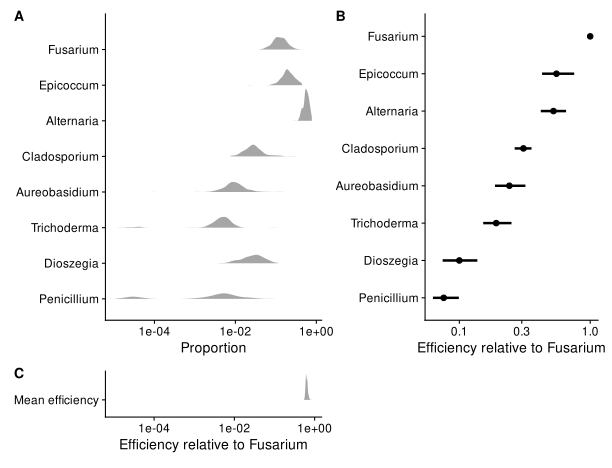
\includegraphics{figures/export-pdf/notebook/_posts/2022-01-08-leopold2020host-case-study/leopold2020host-case-study_files/figure-html5/variation-in-proportions-and-mean-efficiency-1.pdf}
\caption{\label{fig:leopold2020host-variation}\textbf{In the pre-infection samples from Leopold and Busby (\protect\hyperlink{ref-leopold2020host}{2020}), multiplicative variation in taxa proportions is much larger than that in the mean efficiency.} Panel A shows the distribution of the proportions of each commensal isolate (denoted by its genus) across all samples collected prior to pathogen inoculation; Panel C shows the distribution of the (estimated) sample mean efficiency across these same samples on the same scale; and Panel B shows the efficiency of each taxon estimated from DNA mock communities as point estimates and 90\% bootstrap percentile confidence intervals. Efficiencies are shown relative to the most efficiently measured taxon (\emph{Fusarium}).}
\end{figure}



\begin{figure}
\centering
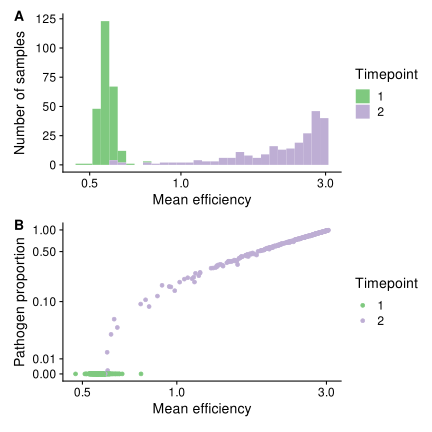
\includegraphics{figures/export-pdf/notebook/_posts/2022-01-08-leopold2020host-case-study/leopold2020host-case-study_files/figure-html5/infection-mean-efficiency-dist-1.pdf}
\caption{\label{fig:leopold2020host-infection-mean-efficiency-dist}\textbf{The mean efficiency tends to increase after infection due to the high proportion of the pathogen.}}
\end{figure}



\begin{figure}
\centering
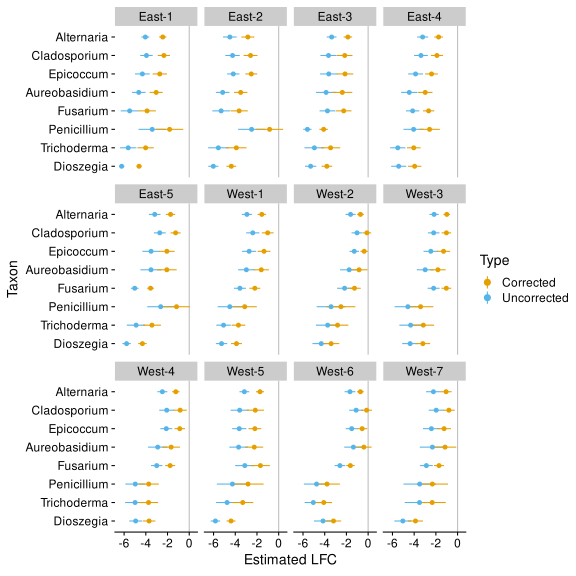
\includegraphics{figures/export-pdf/notebook/_posts/2022-01-08-leopold2020host-case-study/leopold2020host-case-study_files/figure-html5/infection-lfc-estimates-1.pdf}
\caption{\label{fig:leopold2020host-infection-lfc}\textbf{Bias correction increases the estimated increase in log proportion in response to infection for commensal taxa across all host genotypes.} Shown are the estimated log fold change (LFC) and 95\% confidence intervals from simple linear regression of log (base e) proportion against experimental timepoint for commensal taxa. Negative values indicate that the proportion of the taxon decreased on average in response to infection, which we expect due to an increase in pathogen abundance and the sum-to-one constraint of proportions. Bias leads to artificially low estimates, as the increased pathogen proportion drives an increase in mean efficiency.}
\end{figure}



\begin{figure}
\centering
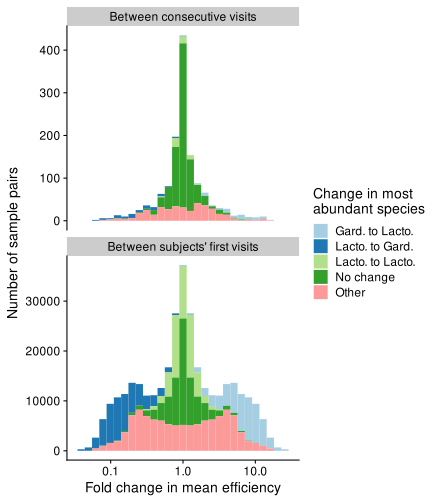
\includegraphics{figures/export-pdf/notebook/_posts/2021-11-01-momspi-summary/momspi-summary_files/figure-html5/momspi-mean-efficiency-fcs-1.pdf}
\caption{\label{fig:momspi-mean-efficiency-fcs}\textbf{Fold changes in the mean efficiency within and between women in the MOMS-PI study.}}
\end{figure}



\begin{figure}
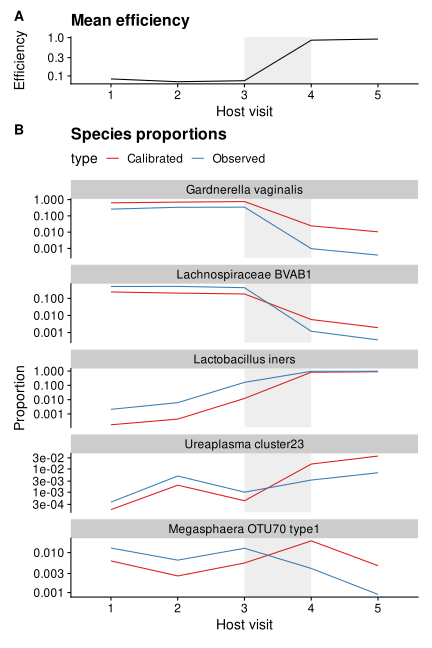
\includegraphics[width=0.75\linewidth]{figures/export-pdf/notebook/_posts/2021-11-01-momspi-summary/momspi-summary_files/figure-html5/trajectories-within-subject-high-var-1} \caption{\textbf{In vaginal microbiome measurements, shifts between \emph{Lactobacillus} and \emph{Gardnerella} dominance can drive spurious fold changes in other, lower-abundance species.} The figure shows species proportions and mean efficiency trajectories over consecutive clinical visits for a subject in the MOMS-PI study whose microbiome samples showed substantial variation in mean efficiency. The subject's samples are dominated by \emph{Gardnerella vaginalis} and \emph{Lachnospiraceae BVAB1} during the first three visits before transitioning to being dominated by \emph{Lactobacillus iners} between visits 3 and 4. This transition drives a sharp increase in the mean efficiency, which significantly distorts the fold changes in the observed (uncalibrated) microbiome measurements for species with less dramatic fold changes. Two exemplar species are shown to illustrate the magnitude (\emph{Ureaplasma cluster 23}) and sign (\emph{Megasphaera OTU70 type1}) errors that can arise in this situation.}\label{fig:momspi-trajectory}
\end{figure}



\begin{figure}
\centering
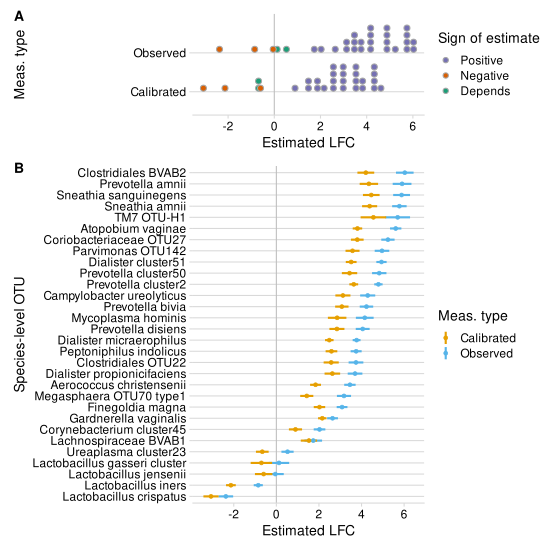
\includegraphics{figures/export-pdf/notebook/_posts/2021-12-15-momspi-regression-diversity/momspi-regression-diversity_files/figure-html5/regression-gp-1.pdf}
\caption{\label{fig:momspi-regression}\textbf{Bias inflates estimated log fold changes (LFCs) in species proportions with diversity in vaginal microbiome samples from the MOMS-PI study.} Samples were split into low, medium, and high diversity groups based on Shannon diversity in observed (uncalibrated) microbiome profiles. The LFC in proportion from low- to high-diversity samples was estimated for 30 common species using gamma-Poisson regression with and without bias correction. Panel A shows the distribution of point estimates; Panel B shows the point estimates and 95\% Bayesian credible intervals for each species.}
\end{figure}



\begin{figure}
\centering
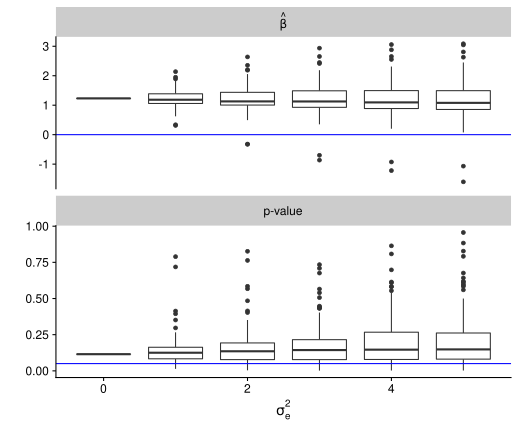
\includegraphics{figures/export-pdf/notebook/_posts/2021-10-18-evaluate-robustness-example/evaluate-robustness-example_files/figure-html5/summary_plot-1.pdf}
\caption{\label{fig:sensitivity-example}\textbf{A bias-sensivity analysis can be performed to examine how sensitive the results of a DA analysis are to assumptions about taxonomic bias in community measurements.} The figure shows the results of a bias-sensitivity analysis used to study the effect of bias on the association of \emph{Gardnerella vaginalis} and preterm birth that was investigated by Callahan et al. (\protect\hyperlink{ref-callahan2017repl}{2017}). 100 random efficiency vectors were drawn at 6 different bias strengths (quantified by the variance in log efficiency, \(\sigma_{e}^{2}\)). Each efficiency vector was used to calibrate the MGS profiles and perform a DA association test of \emph{G. vaginalis} versus the host's preterm birth outcome; regression coefficients \(\hat \beta\) indicate the increase of average logit proportion of \emph{G. vaginalis} in women who experienced preterm birth.}
\end{figure}



\hypertarget{references}{%
\section*{References}\label{references}}
\addcontentsline{toc}{section}{References}

\hypertarget{refs}{}
\begin{CSLReferences}{1}{0}
\leavevmode\vadjust pre{\hypertarget{ref-barlow2020aqau}{}}%
Barlow, Jacob T., Said R. Bogatyrev, and Rustem F. Ismagilov. 2020. {``{A quantitative sequencing framework for absolute abundance measurements of mucosal and lumenal microbial communities}.''} \emph{Nat. Commun.} 11 (1): 1--13. \url{https://doi.org/10.1038/s41467-020-16224-6}.

\leavevmode\vadjust pre{\hypertarget{ref-brooks2015thet}{}}%
Brooks, J Paul, David J Edwards, Michael D Harwich, Maria C Rivera, Jennifer M Fettweis, Myrna G Serrano, Robert A Reris, et al. 2015. {``{The truth about metagenomics: quantifying and counteracting bias in 16S rRNA studies}.''} \emph{BMC Microbiol.} BioMed Central. \url{https://doi.org/10.1186/s12866-015-0351-6}.

\leavevmode\vadjust pre{\hypertarget{ref-callahan2017repl}{}}%
Callahan, Benjamin J, Daniel B DiGiulio, Daniela S Aliaga Goltsman, Christine L Sun, Elizabeth K Costello, Pratheepa Jeganathan, Joseph R Biggio, et al. 2017. {``{Replication and refinement of a vaginal microbial signature of preterm birth in two racially distinct cohorts of US women}.''} \emph{Proc. Natl. Acad. Sci. U. S. A.} 114 (37): 9966--71. \url{https://doi.org/10.1073/pnas.1705899114}.

\leavevmode\vadjust pre{\hypertarget{ref-cartwright2018mult}{}}%
Cartwright, Charles P., Amanda J. Pherson, Ayla B. Harris, Matthew S. Clancey, and Melinda B. Nye. 2018. {``{Multicenter study establishing the clinical validity of a nucleic-acid amplification--based assay for the diagnosis of bacterial vaginosis}.''} \emph{Diagn. Microbiol. Infect. Dis.} 92 (3): 173--78. \url{https://doi.org/10.1016/j.diagmicrobio.2018.05.022}.

\leavevmode\vadjust pre{\hypertarget{ref-chng2020meta}{}}%
Chng, Kern Rei, Tarini Shankar Ghosh, Yi Han Tan, Tannistha Nandi, Ivor Russel Lee, Amanda Hui Qi Ng, Chenhao Li, et al. 2020. {``{Metagenome-wide association analysis identifies microbial determinants of post-antibiotic ecological recovery in the gut}.''} \emph{Nat. Ecol. Evol.} 4 (9): 1256--67. \url{https://doi.org/10.1038/s41559-020-1236-0}.

\leavevmode\vadjust pre{\hypertarget{ref-contijoch2019gutm}{}}%
Contijoch, Eduardo J, Graham J Britton, Chao Yang, Ilaria Mogno, Zhihua Li, Ruby Ng, Sean R Llewellyn, et al. 2019. {``{Gut microbiota density influences host physiology and is shaped by host and microbial factors}.''} \emph{Elife} 8 (January). \url{https://doi.org/10.7554/eLife.40553}.

\leavevmode\vadjust pre{\hypertarget{ref-cruz2021equi}{}}%
Cruz, Giuliano Netto Flores, Ana Paula Christoff, and Luiz Felipe Valter de Oliveira. 2021. {``{Equivolumetric Protocol Generates Library Sizes Proportional to Total Microbial Load in 16S Amplicon Sequencing}.''} \emph{Front. Microbiol.} 12 (February): 1--16. \url{https://doi.org/10.3389/fmicb.2021.638231}.

\leavevmode\vadjust pre{\hypertarget{ref-david2014host}{}}%
David, Lawrence A, Arne C Materna, Jonathan Friedman, Maria I Campos-Baptista, Matthew C Blackburn, Allison Perrotta, Susan E Erdman, and Eric J Alm. 2014. {``{Host lifestyle affects human microbiota on daily timescales}.''} \emph{Genome Biol.} 15 (7): R89. \url{https://doi.org/10.1186/gb-2014-15-7-r89}.

\leavevmode\vadjust pre{\hypertarget{ref-diener2021nonr}{}}%
Diener, Christian, Anna C. H. Hoge, Sean M. Kearney, Ulrike Kusebauch, Sushmita Patwardhan, Robert L. Moritz, Susan E. Erdman, and Sean M. Gibbons. 2021. {``{Non-responder phenotype reveals apparent microbiome-wide antibiotic tolerance in the murine gut}.''} \emph{Commun. Biol.} 4 (1). \url{https://doi.org/10.1038/s42003-021-01841-8}.

\leavevmode\vadjust pre{\hypertarget{ref-dreo2014opti}{}}%
Dreo, Tanja, Manca Pirc, Živa Ramšak, Jernej Pavšič, Mojca Milavec, Jana Žel, and Kristina Gruden. 2014. {``{Optimising droplet digital PCR analysis approaches for detection and quantification of bacteria: a case study of fire blight and potato brown rot}.''} \emph{Anal. Bioanal. Chem.} 406 (26): 6513--28. \url{https://doi.org/10.1007/s00216-014-8084-1}.

\leavevmode\vadjust pre{\hypertarget{ref-fettweis2019thev}{}}%
Fettweis, Jennifer M., Myrna G. Serrano, Jamie Paul Brooks, David J. Edwards, Philippe H. Girerd, Hardik I. Parikh, Bernice Huang, et al. 2019. {``{The vaginal microbiome and preterm birth}.''} \emph{Nat. Med.} 25 (6): 1012--21. \url{https://doi.org/10.1038/s41591-019-0450-2}.

\leavevmode\vadjust pre{\hypertarget{ref-finucane2014atax}{}}%
Finucane, Mariel M., Thomas J. Sharpton, Timothy J. Laurent, and Katherine S. Pollard. 2014. {``{A Taxonomic Signature of Obesity in the Microbiome? Getting to the Guts of the Matter}.''} Edited by Markus M. Heimesaat. \emph{PLoS One} 9 (1): e84689. \url{https://doi.org/10.1371/journal.pone.0084689}.

\leavevmode\vadjust pre{\hypertarget{ref-galazzo2020howt}{}}%
Galazzo, Gianluca, Niels van Best, Birke J. Benedikter, Kevin Janssen, Liene Bervoets, Christel Driessen, Melissa Oomen, et al. 2020. {``{How to Count Our Microbes? The Effect of Different Quantitative Microbiome Profiling Approaches}.''} \emph{Front. Cell. Infect. Microbiol.} 10 (August). \url{https://doi.org/10.3389/fcimb.2020.00403}.

\leavevmode\vadjust pre{\hypertarget{ref-gill2016eval}{}}%
Gill, Christina, Janneke H. H. M. van de Wijgert, Frances Blow, and Alistair C. Darby. 2016. {``{Evaluation of Lysis Methods for the Extraction of Bacterial DNA for Analysis of the Vaginal Microbiota}.''} Edited by Peter E. Larsen. \emph{PLoS One} 11 (9): e0163148. \url{https://doi.org/10.1371/journal.pone.0163148}.

\leavevmode\vadjust pre{\hypertarget{ref-gloor2017micr}{}}%
Gloor, Gregory B., Jean M. Macklaim, Vera Pawlowsky-Glahn, and Juan J. Egozcue. 2017. {``{Microbiome Datasets Are Compositional: And This Is Not Optional}.''} \emph{Front. Microbiol.} 8 (November): 2224. \url{https://doi.org/10.3389/fmicb.2017.02224}.

\leavevmode\vadjust pre{\hypertarget{ref-graspeuntner2018sele}{}}%
Graspeuntner, Simon, Nathalie Loeper, Sven Künzel, John F. Baines, and Jan Rupp. 2018. {``{Selection of validated hypervariable regions is crucial in 16S-based microbiota studies of the female genital tract}.''} \emph{Sci. Rep.} 8 (1): 9678. \url{https://doi.org/10.1038/s41598-018-27757-8}.

\leavevmode\vadjust pre{\hypertarget{ref-hardwick2018synt}{}}%
Hardwick, Simon A., Wendy Y. Chen, Ted Wong, Bindu S. Kanakamedala, Ira W. Deveson, Sarah E. Ongley, Nadia S. Santini, et al. 2018. {``{Synthetic microbe communities provide internal reference standards for metagenome sequencing and analysis}.''} \emph{Nat. Commun.} 9 (1): 3096. \url{https://doi.org/10.1038/s41467-018-05555-0}.

\leavevmode\vadjust pre{\hypertarget{ref-harrison2021theq}{}}%
Harrison, Joshua G., W. John Calder, Bryan Shuman, and C. Alex Buerkle. 2021. {``{The quest for absolute abundance: The use of internal standards for DNA‐based community ecology}.''} \emph{Mol. Ecol. Resour.} 21 (1): 30--43. \url{https://doi.org/10.1111/1755-0998.13247}.

\leavevmode\vadjust pre{\hypertarget{ref-huttenhower2012stru}{}}%
Huttenhower, Curtis, Dirk Gevers, Rob Knight, Sahar Abubucker, Jonathan H. Badger, Asif T. Chinwalla, Heather H. Creasy, et al. 2012. {``{Structure, function and diversity of the healthy human microbiome}.''} \emph{Nature} 486 (7402): 207--14. \url{https://doi.org/10.1038/nature11234}.

\leavevmode\vadjust pre{\hypertarget{ref-ji2019quan}{}}%
Ji, Brian W., Ravi U. Sheth, Purushottam D. Dixit, Yiming Huang, Andrew Kaufman, Harris H. Wang, and Dennis Vitkup. 2019. {``{Quantifying spatiotemporal variability and noise in absolute microbiota abundances using replicate sampling}.''} \emph{Nat. Methods} 16 (8): 731--36. \url{https://doi.org/10.1038/s41592-019-0467-y}.

\leavevmode\vadjust pre{\hypertarget{ref-jian2020quan}{}}%
Jian, Ching, Panu Luukkonen, Hannele Yki-Järvinen, Anne Salonen, and Katri Korpela. 2020. {``{Quantitative PCR provides a simple and accessible method for quantitative microbiota profiling}.''} Edited by Ivone Vaz-Moreira. \emph{PLoS One} 15 (1): e0227285. \url{https://doi.org/10.1371/journal.pone.0227285}.

\leavevmode\vadjust pre{\hypertarget{ref-karasov2020ther}{}}%
Karasov, Talia L., Manuela Neumann, Alejandra Duque-Jaramillo, Sonja Kersten, Ilja Bezrukov, Birgit Schröppel, Efthymia Symeonidi, et al. 2020. {``{The relationship between microbial population size and disease in the Arabidopsis thaliana phyllosphere}.''} \emph{bioRxiv}. \url{https://doi.org/10.1101/828814}.

\leavevmode\vadjust pre{\hypertarget{ref-kevorkian2018esti}{}}%
Kevorkian, Richard, Jordan T Bird, Alexander Shumaker, and Karen G Lloyd. 2018. {``{Estimating Population Turnover Rates by Relative Quantification Methods Reveals Microbial Dynamics in Marine Sediment}.''} \emph{Appl. Environ. Microbiol.} 84 (1): e01443--17. \url{https://doi.org/10.1128/AEM.01443-17}.

\leavevmode\vadjust pre{\hypertarget{ref-korpela2018inte}{}}%
Korpela, Katri, Elin W. Blakstad, Sissel J. Moltu, Kenneth Strømmen, Britt Nakstad, Arild E. Rønnestad, Kristin Brække, Per O. Iversen, Christian A. Drevon, and Willem de Vos. 2018. {``{Intestinal microbiota development and gestational age in preterm neonates}.''} \emph{Sci. Rep.} 8 (1): 1--9. \url{https://doi.org/10.1038/s41598-018-20827-x}.

\leavevmode\vadjust pre{\hypertarget{ref-kumar2018anal}{}}%
Kumar, M. Senthil, Eric V. Slud, Kwame Okrah, Stephanie C. Hicks, Sridhar Hannenhalli, and Héctor Corrada Bravo. 2018. {``{Analysis and correction of compositional bias in sparse sequencing count data}.''} \emph{BMC Genomics} 19 (1): 799. \url{https://doi.org/10.1186/s12864-018-5160-5}.

\leavevmode\vadjust pre{\hypertarget{ref-leopold2020host}{}}%
Leopold, Devin R, and Posy E Busby. 2020. {``{Host Genotype and Colonist Arrival Order Jointly Govern Plant Microbiome Composition and Function}.''} \emph{Curr. Biol.} 30 (16): 3260--3266.e5. \url{https://doi.org/10.1016/j.cub.2020.06.011}.

\leavevmode\vadjust pre{\hypertarget{ref-lloyd2020evid}{}}%
Lloyd, Karen G., Jordan T. Bird, Joy Buongiorno, Emily Deas, Richard Kevorkian, Talor Noordhoek, Jacob Rosalsky, and Taylor Roy. 2020. {``{Evidence for a Growth Zone for Deep-Subsurface Microbial Clades in Near-Surface Anoxic Sediments}.''} \emph{Appl. Environ. Microbiol.} 86 (19): 1--15. \url{https://doi.org/10.1128/AEM.00877-20}.

\leavevmode\vadjust pre{\hypertarget{ref-lloyd2013meta}{}}%
Lloyd, Karen G., Megan K. May, Richard T. Kevorkian, and Andrew D. Steen. 2013. {``{Meta-analysis of quantification methods shows that archaea and bacteria have similar abundances in the subseafloor}.''} \emph{Appl. Environ. Microbiol.} 79 (24): 7790--99. \url{https://doi.org/10.1128/AEM.02090-13}.

\leavevmode\vadjust pre{\hypertarget{ref-lofgren2019geno}{}}%
Lofgren, Lotus A., Jessie K. Uehling, Sara Branco, Thomas D. Bruns, Francis Martin, and Peter G. Kennedy. 2019. {``{Genome‐based estimates of fungal rDNA copy number variation across phylogenetic scales and ecological lifestyles}.''} \emph{Mol. Ecol.} 28 (4): 721--30. \url{https://doi.org/10.1111/mec.14995}.

\leavevmode\vadjust pre{\hypertarget{ref-lozupone2013meta}{}}%
Lozupone, Catherine A, Jesse Stombaugh, Antonio Gonzalez, Gail Ackermann, Janet K Jansson, Jeffrey I Gordon, Doug Wendel, Yoshiki Va, and Rob Knight. 2013. {``{Meta-analyses of studies of the human microbiota}.''} \emph{Genome Res.}, 1704--14. \url{https://doi.org/10.1101/gr.151803.112}.

\leavevmode\vadjust pre{\hypertarget{ref-mandal2015anal}{}}%
Mandal, Siddhartha, Will Van Treuren, Richard A. White, Merete Eggesbø, Rob Knight, and Shyamal D. Peddada. 2015. {``{Analysis of composition of microbiomes: a novel method for studying microbial composition}.''} \emph{Microb. Ecol. Heal. Dis.} 26 (1): 27663. \url{https://doi.org/10.3402/mehd.v26.27663}.

\leavevmode\vadjust pre{\hypertarget{ref-mclaren2019cons}{}}%
McLaren, Michael R, Amy D Willis, and Benjamin J Callahan. 2019. {``{Consistent and correctable bias in metagenomic sequencing experiments}.''} \emph{Elife} 8 (September): 46923. \url{https://doi.org/10.7554/eLife.46923}.

\leavevmode\vadjust pre{\hypertarget{ref-morella2018rapi}{}}%
Morella, Norma M., Shangyang Christopher Yang, Catherine A. Hernandez, and Britt Koskella. 2018. {``{Rapid quantification of bacteriophages and their bacterial hosts in vitro and in vivo using droplet digital PCR}.''} \emph{J. Virol. Methods} 259 (May): 18--24. \url{https://doi.org/10.1016/j.jviromet.2018.05.007}.

\leavevmode\vadjust pre{\hypertarget{ref-pavsic2016digi}{}}%
Pavšič, Jernej, Jana Žel, and Mojca Milavec. 2016. {``{Digital PCR for direct quantification of viruses without DNA extraction}.''} \emph{Anal. Bioanal. Chem.} 408 (1): 67--75. \url{https://doi.org/10.1007/s00216-015-9109-0}.

\leavevmode\vadjust pre{\hypertarget{ref-props2017abso}{}}%
Props, Ruben, Frederiek-Maarten Kerckhof, Peter Rubbens, Jo De Vrieze, Emma Hernandez Sanabria, Willem Waegeman, Pieter Monsieurs, Frederik Hammes, and Nico Boon. 2017. {``{Absolute quantification of microbial taxon abundances}.''} \emph{ISME J.} 11 (2): 584--87. \url{https://doi.org/10.1038/ismej.2016.117}.

\leavevmode\vadjust pre{\hypertarget{ref-rao2021mult}{}}%
Rao, Chitong, Katharine Z. Coyte, Wayne Bainter, Raif S. Geha, Camilia R. Martin, and Seth Rakoff-Nahoum. 2021. {``{Multi-kingdom ecological drivers of microbiota assembly in preterm infants}.''} \emph{Nature} 591 (7851): 633--38. \url{https://doi.org/10.1038/s41586-021-03241-8}.

\leavevmode\vadjust pre{\hypertarget{ref-regalado2019comb}{}}%
Regalado, Julian, Derek S. Lundberg, Oliver Deusch, Sonja Kersten, Talia Karasov, Karin Poersch, Gautam Shirsekar, and Detlef Weigel. 2020. {``{Combining whole-genome shotgun sequencing and rRNA gene amplicon analyses to improve detection of microbe--microbe interaction networks in plant leaves}.''} \emph{ISME J.}, May, 823492. \url{https://doi.org/10.1038/s41396-020-0665-8}.

\leavevmode\vadjust pre{\hypertarget{ref-smets2016amet}{}}%
Smets, Wenke, Jonathan W. Leff, Mark A. Bradford, Rebecca L. McCulley, Sarah Lebeer, and Noah Fierer. 2016. {``{A method for simultaneous measurement of soil bacterial abundances and community composition via 16S rRNA gene sequencing}.''} \emph{Soil Biol. Biochem.} 96: 145--51. \url{https://doi.org/10.1016/j.soilbio.2016.02.003}.

\leavevmode\vadjust pre{\hypertarget{ref-srinivasan2012bact}{}}%
Srinivasan, Sujatha, Noah G. Hoffman, Martin T. Morgan, Frederick A. Matsen, Tina L. Fiedler, Robert W. Hall, Frederick J. Ross, et al. 2012. {``{Bacterial Communities in Women with Bacterial Vaginosis: High Resolution Phylogenetic Analyses Reveal Relationships of Microbiota to Clinical Criteria}.''} Edited by Adam J. Ratner. \emph{PLoS One} 7 (6): e37818. \url{https://doi.org/10.1371/journal.pone.0037818}.

\leavevmode\vadjust pre{\hypertarget{ref-stammler2016adju}{}}%
Stämmler, Frank, Joachim Gläsner, Andreas Hiergeist, Ernst Holler, Daniela Weber, Peter J. Oefner, André Gessner, and Rainer Spang. 2016. {``{Adjusting microbiome profiles for differences in microbial load by spike-in bacteria}.''} \emph{Microbiome} 4 (1): 28. \url{https://doi.org/10.1186/s40168-016-0175-0}.

\leavevmode\vadjust pre{\hypertarget{ref-tettamantiboshier2020comp}{}}%
Tettamanti Boshier, Florencia A., Sujatha Srinivasan, Anthony Lopez, Noah G. Hoffman, Sean Proll, David N. Fredricks, and Joshua T. Schiffer. 2020. {``{Complementing 16S rRNA Gene Amplicon Sequencing with Total Bacterial Load To Infer Absolute Species Concentrations in the Vaginal Microbiome}.''} \emph{mSystems} 5 (2): 1--14. \url{https://doi.org/10.1128/mSystems.00777-19}.

\leavevmode\vadjust pre{\hypertarget{ref-tkacz2018abso}{}}%
Tkacz, Andrzej, Marion Hortala, and Philip S. Poole. 2018. {``{Absolute quantitation of microbiota abundance in environmental samples}.''} \emph{Microbiome} 6 (1): 110. \url{https://doi.org/10.1186/s40168-018-0491-7}.

\leavevmode\vadjust pre{\hypertarget{ref-vandeputte2017quan}{}}%
Vandeputte, Doris, Gunter Kathagen, Kevin D'hoe, Sara Vieira-Silva, Mireia Valles-Colomer, João Sabino, Jun Wang, et al. 2017. {``{Quantitative microbiome profiling links gut community variation to microbial load}.''} \emph{Nature} 551 (7681): 507. \url{https://doi.org/10.1038/nature24460}.

\leavevmode\vadjust pre{\hypertarget{ref-vaninsberghe2020diar}{}}%
VanInsberghe, David, Joseph A. Elsherbini, Bernard Varian, Theofilos Poutahidis, Susan Erdman, and Martin F. Polz. 2020. {``{Diarrhoeal events can trigger long-term Clostridium difficile colonization with recurrent blooms}.''} \emph{Nat. Microbiol.} 5 (4): 642--50. \url{https://doi.org/10.1038/s41564-020-0668-2}.

\leavevmode\vadjust pre{\hypertarget{ref-vieirasilva2019quan}{}}%
Vieira-Silva, Sara, João Sabino, Mireia Valles-Colomer, Gwen Falony, Gunter Kathagen, Clara Caenepeel, Isabelle Cleynen, Schalk van der Merwe, Séverine Vermeire, and Jeroen Raes. 2019. {``{Quantitative microbiome profiling disentangles inflammation- and bile duct obstruction-associated microbiota alterations across PSC/IBD diagnoses}.''} \emph{Nat. Microbiol.} 4 (11): 1826--31. \url{https://doi.org/10.1038/s41564-019-0483-9}.

\leavevmode\vadjust pre{\hypertarget{ref-wallace2021thed}{}}%
Wallace, Megan A., Kelsey A. Coffman, Clément Gilbert, Sanjana Ravindran, Gregory F. Albery, Jessica Abbott, Eliza Argyridou, et al. 2021. {``{The discovery, distribution, and diversity of DNA viruses associated with Drosophila melanogaster in Europe}.''} \emph{Virus Evol.} 7 (1): 1--23. \url{https://doi.org/10.1093/ve/veab031}.

\leavevmode\vadjust pre{\hypertarget{ref-wang2021curr}{}}%
Wang, Xiaofan, Samantha Howe, Feilong Deng, and Jiangchao Zhao. 2021. {``{Current Applications of Absolute Bacterial Quantification in Microbiome Studies and Decision-Making Regarding Different Biological Questions}.''} \emph{Microorganisms} 9 (9): 1797. \url{https://doi.org/10.3390/microorganisms9091797}.

\leavevmode\vadjust pre{\hypertarget{ref-wasserman2004allo}{}}%
Wasserman, Larry. 2004. \emph{{All of Statistics}}. Springer Texts in Statistics. New York, NY: Springer New York. \url{https://doi.org/10.1007/978-0-387-21736-9}.

\leavevmode\vadjust pre{\hypertarget{ref-yeh2018taxo}{}}%
Yeh, Yi-Chun, David M. Needham, Ella T. Sieradzki, and Jed A. Fuhrman. 2018. {``{Taxon Disappearance from Microbiome Analysis Reinforces the Value of Mock Communities as a Standard in Every Sequencing Run}.''} \emph{mSystems} 3 (3): e00023--18. \url{https://doi.org/10.1128/mSystems.00023-18}.

\leavevmode\vadjust pre{\hypertarget{ref-yuan2012eval}{}}%
Yuan, Sanqing, Dora B. Cohen, Jacques Ravel, Zaid Abdo, and Larry J. Forney. 2012. {``{Evaluation of Methods for the Extraction and Purification of DNA from the Human Microbiome}.''} Edited by Jack Anthony Gilbert. \emph{PLoS One} 7 (3): e33865. \url{https://doi.org/10.1371/journal.pone.0033865}.

\leavevmode\vadjust pre{\hypertarget{ref-zemb2020abso}{}}%
Zemb, Olivier, Caroline S Achard, Jerome Hamelin, Marie‐Léa De Almeida, Béatrice Gabinaud, Laurent Cauquil, Lisanne M. G. Verschuren, and Jean-jacques Godon. 2020. {``{Absolute quantitation of microbes using 16S rRNA gene metabarcoding: A rapid normalization of relative abundances by quantitative PCR targeting a 16S rRNA gene spike‐in standard}.''} \emph{Microbiologyopen} 9 (3): 1--21. \url{https://doi.org/10.1002/mbo3.977}.

\leavevmode\vadjust pre{\hypertarget{ref-zhang2017soil}{}}%
Zhang, Zhaojing, Yuanyuan Qu, Shuzhen Li, Kai Feng, Shang Wang, Weiwei Cai, Yuting Liang, et al. 2017. {``{Soil bacterial quantification approaches coupling with relative abundances reflecting the changes of taxa}.''} \emph{Sci. Rep.} 7 (1): 1--11. \url{https://doi.org/10.1038/s41598-017-05260-w}.

\end{CSLReferences}

\end{document}
